\chapter{Transport à longue portée dans la classe CDP}

\label{chapter:TransportLP}

\subparagraph{}Dans le chapitre précédent, nous avons présenté la classe CDP comme une classe d'universalité recouvrant potentiellement un grand nombre de transitions de phase absorbantes. Un système appartenant à cette classe est décrit par un ensemble de comportements et d'exposants critiques caractéristiques de la criticalité associée. Par exemple, en notant $\langle A \rangle$ l'activité moyenne dans le système, $\langle \delta A^2 \rangle$ ses fluctuations, $\xi$ la longueur de corrélation et $\epsilon$ la distance au point critique, les exposants $\beta$, $\gamma^\prime$ et $\nu_\perp$ permettent de définir les évolutions suivantes proche de la transition :

\begin{equation}
	\langle A \rangle \sim \epsilon^\beta, \quad \langle \delta A^2 \rangle \sim \epsilon^{-\gamma^\prime}, \quad \xi \sim \epsilon^{-\nu_\perp}.
\end{equation}

\noindent Ces exposants sont connus exactement dans l'approximation de champ moyen avec $\beta^\text{CM} = 1$, $\gamma^{\prime\text{CM}} = 0$, $\nu_\perp^\text{CM} = \frac{1}{2}$. En dimension finie $D<4$ et en présence d'interactions à courte portée uniquement, les exposants critiques ont été mesurés numériquement \cite{lubeck_universal_2004} et calculés analytiquement, de manière perturbative, via les méthodes du groupe de renormalisation fonctionnel appliquées à la transition de dépiégeage.

\subparagraph{}Comme nous l'avons mentionné au \autoref{chapter:introduction}, la présence d'interactions à longue portée dans les modèles représentant des phénomènes critiques permet en général de passer du comportement critique de dimension finie au comportement critique de champ moyen de la classe d'universalité associée. Dans ce chapitre, nous proposons de définir plus précisément ce cadre générique associé à l'universalité CDP. L'établissement de ce cadre est un objet central dans notre travail puisqu'il nous permettra, par contraste, d'interpréter le comportement atypique des transitions de réversibilité et d'écoulement dans les chapitres suivants.

\subparagraph{}Pour ce faire, nous commencerons par identifier ce cadre, que nous baptisons LR-CDP pour \textit{long-range conserved directed percolation}, d'un point de vue théorique. S'appuyant sur des résultats pré-existants, cette première analyse permettra de définir l'évolution du comportement critique attendue avec la portée des interactions. Nous verrons par ailleurs que, dans ce cadre naturel d'extension de la théorie CDP, les interactions à longue portée représentent un transport à longue portée de la quantité conservé sous l'influence locale de l'activité. Afin de disposer d'un socle de comparaison solide, nous préciserons dans un second temps ce cadre théorique via une approche numérique. Cette caractérisation se fera via l'étude des modèles Manna et ROM et leur extension au cadre LR-CDP en 2D, dimension dans laquelle nous étudierons les transitions de réversibilité et d'écoulement par la suite. Cette analyse sera menée via la détermination des exposants critiques statiques et dynamiques associés et l'évolution des propriétés d'hyperuniformité avec la portée du transport.

\section{Longue portée et comportement critique}

\subparagraph{}Dans cette section, nous présentons le cadre générique de compréhension des interactions à longue portée dans le cas de la criticalité CDP. Après avoir explicité la phénoménologie globale induite par la présence de ce type d'interactions, nous présenterons l'extension naturelle de la théorie CDP via la modification des équations de champ associées. Celle-ci nous permettra alors de déterminer un comportement qualitatif attendu quant à l'évolution de chaque exposant critique avec l'exposant de portée $\alpha$, soutenue par des calculs analytiques pré-existants.

\label{sec:LRCanonique}

\subsection{Phénoménologie}

\subparagraph{}Dans de nombreux systèmes de physique statistique faisant intervenir des transitions de phase, les interactions entre agents prennent un caractère non-local. Dans la plupart de ces cas, cette non-localité peut-être représentée par des interactions décroissant algébriquement avec la distance $r$ séparant les agents, soit comme $\sim 1/r^\alpha$ avec $\alpha >0$. On peut par exemple penser aux interactions de Coulomb entre deux charges ou aux interactions gravitationnelles entre deux masses qui décroissent comme $\sim 1/r$ en trois dimensions, soit $\alpha = 1$. 

\subparagraph{}Comme nous l'avons vu précédemment, dans la limite $\alpha \rightarrow 0$ un système adopte naturellement le comportement critique équivalent au champ moyen de la classe d'universalité associée. \`A l'inverse, dans la limite $\alpha \rightarrow \infty$, ce système adopte le comportement critique de la classe en dimension finie. En fait, dans le cas général, ces deux comportements limites ne prennent pas uniquement place pour des formes asymptotiques de la portée d'interaction. \`A la place, il est possible d'identifier deux bornes $\alpha^+$ et $\alpha^-$ définissant deux zones. Dans toute la gamme d'exposants $\alpha>\alpha^+$, le système présente son comportement critique de courte portée, associé au cas faisant intervenir des interactions locales uniquement. De la même façon, dans toute la gamme d'exposants $\alpha < \alpha^-$, le comportement critique mesuré est celui du champ moyen associé.

\begin{figure}[h]
	\centering
	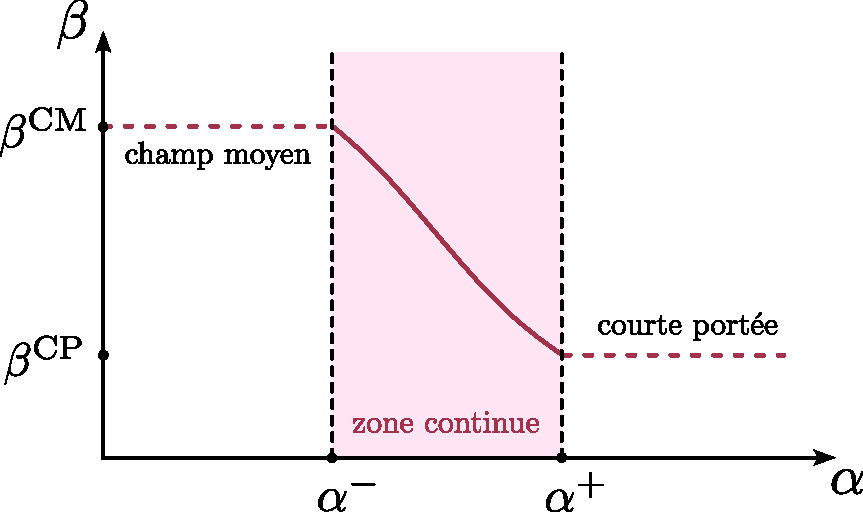
\includegraphics[width=0.7\textwidth]{Chapitre1/Figures/LongRange/beta_base.pdf}
	\caption{Évolution générique de l'exposant $\beta$ avec la portée d'interaction. $\beta^\text{CP}$ est l'exposant attendu dans un modèle avec interactions locales et $\beta^\text{CM}$ est l'exposant attendu dans le cas champ moyen. Cette évolution générique est retrouvée pour les autres exposants critiques.}
	\label{fig:exp_base}
\end{figure}

\subparagraph{}Dans le cas d'une portée intermédiaire $\alpha^- < \alpha < \alpha^+$, plusieurs scénarios sont intuitivement possibles. En fait, ce que l'on observe et rationalise c'est qu'entre ces deux bornes, le comportement critique évolue continûment avec la portée. Chaque exposant critique prend une valeur unique dépendant uniquement de la portée $\alpha$, reliant une valeur de courte portée pour $\alpha = \alpha^+$ à une valeur de champ moyen pour $\alpha = \alpha^-$, comme représenté à la \autoref{fig:exp_base}. Ainsi, il est possible de définir une infinité continue de classes d'universalité associées à celle de courte portée.

\subparagraph{}Cette phénoménologie ayant un caractère général général, retrouvée aussi bien dans les cas d'équilibre que dans les cas hors d'équilibre, nous cherchons à la préciser dans le cas de la classe d'universalité CDP.

\subsection{Formulation théorique dans la classe CDP}

\paragraph{Équations de champ et transport à longue portée}

\subparagraph{}Il est possible de comprendre la phénoménologie liée à l'ajout d'interactions à longue portée via les théories continues associées aux phénomènes critiques. Généralement, dans le cas de la présence d'interactions à longue portée, les équations de champ sont modifiées par l'ajout de termes d'interaction généralisés. Là où les interactions locales sont représentées par l'opérateur laplacien $\nabla^2$, représenté par un terme en $\sim -q^2$ dans l'espace réciproque, les interactions non-locales sont représentées par l'opérateur de dérivée fractionnaire $|\nabla|^{\alpha-D}$, représenté par un terme en $\sim |q|^{\alpha-D}$ dans l'espace réciproque \cite{hinrichsen_non_equilibrium_2007}. Dans le cas de la théorie de champ CDP, les équations généralisées prennent donc la forme :

\begin{equation}
\begin{aligned}
	\partial_t A(\mathbf{r}, t) &= (\omega\rho (\mathbf{r}, t) - r)A(\mathbf{r}, t) - uA^2(\mathbf{r}, t) + \kappa\nabla^2 A (\mathbf{r}, t) \\
	&- \kappa_\alpha|\nabla|^{\alpha-D} A (\mathbf{r}, t) + \sigma \sqrt{A(\mathbf{r}, t)} \eta(\mathbf{r}, t),\\
	\partial_t \rho (\mathbf{r}, t) &= \kappa\nabla^2 A (\mathbf{r}, t)- \kappa_\alpha|\nabla|^{\alpha-D} A (\mathbf{r}, t),
\end{aligned}
\label{eq:LRCDP}
\end{equation}

\noindent avec :

\begin{equation}
	|\nabla|^{\alpha-D} A (\mathbf{r}, t) \propto \int \mathrm{d}\mathbf{r}^\prime ~ \frac{A(\mathbf{r}+\mathbf{r}^\prime)-A(\mathbf{r})}{|\mathbf{r}^{\prime}|^{\alpha}}.
\end{equation}

\noindent On appellera cette théorie LR-CDP pour \textit{long-range conserved directed percolation}. Il est à noter que ce type de cadre théorique n'est pas propre à cette classe, on le retrouve génériquement pour les autres théories comme la théorie $\phi^4$ ou la théorie DP \cite{fisher_critical_1972, hinrichsen_non_equilibrium_2007}.

\subparagraph{}Dans le cadre de la théorie CDP, cette modification continue peut donc se comprendre directement comme une modification des modalités de redistribution. Là où le laplacien signifiait une redistribution des particules (ou de la force élastique dans le cas de la transition de dépiégeage) induit localement par l'activité dans le voisinage proche, le laplacien fractionnaire modélise une redistribution à longue portée, caractérisée par l'exposant $\alpha$. Dans le cadre théorique LR-CDP, la longue portée se comprend donc comme un transport à longue portée induit localement par l'activité. Dans le cas des modèles de particules, il se traduit comme une distribution $P(\mathbf{r}^\prime)\sim 1/|\mathbf{r}^{\prime}|^{\alpha}$ des sauts $\mathbf{r}^{\prime}$ des particules actives. Dans le cas de la transition de dépiégeage, il se matérialise via le propagateur de redistribution élastique $\mathcal{G}(\mathbf{r})\sim 1/|\mathbf{r}|^\alpha$. Pour ces raisons, nous préférerons parler de transport à longue portée plus que d'interactions à longue portée dans le cadre LR-CDP.

\paragraph{Zone continue d'évolution des exposants}

\subparagraph{}Pour déterminer les bornes $\alpha^+$ et $\alpha^-$ dans le cadre de la théorie LR-CDP, nous pouvons raisonner sur des arguments d'échelle.

\subparagraph{}Par définition, la borne de courte portée $\alpha^+$ résulte d'une compétition entre le terme d'interaction local en $\nabla^2 A$ et le terme d'interaction à longue portée en $|\nabla|^{\alpha-D} A$. Pour comparer l'importance de ces deux termes, il est plus simple de raisonner dans l'espace réciproque. Dans ce cas, l'interaction locale est représentée par un terme en $\sim q^2$ tandis que l'interaction non-locale par in terme en $\sim |q|^{\alpha-D}$. \`A grande échelle ($q \rightarrow 0$), le terme local prédomine donc dans la limite $\alpha > D+2$ alors que le terme non-local l'emporte pour $\alpha < D+2$. Ainsi, on a $\alpha^+ = D+2$. Dans le cas qui nous intéresse, en deux dimensions, nous nous attendons donc à ce que l'interaction à longue portée affecte le comportement critique seulement pour $\alpha < 4$. En-deçà de cette portée ($\alpha > 4$), on retrouve le comportement habituel de la classe CDP en 2D.

\subparagraph{}Pour identifier la borne $\alpha^-$, nous pouvons mener une analyse d'échelle sur l'\autoref{eq:LRCDP} pour déterminer la dimension critique supérieure associée, de la même manière que dans la théorie $\phi^4$ ou DP à courte portée (voir \autoref{sec:univcritique}). En gardant en mémoire que le terme d'interaction pertinent dans ce cas est le terme non-local, nous trouvons simplement :

\begin{equation}
	D_c = 2(\alpha-D),\quad \nu_\parallel^\text{CM}= \beta^\text{CM}= 1, \quad \nu_\perp^\text{CM}=\frac{1}{\alpha-D}.
\end{equation}

\noindent Par définition on a $\alpha = \alpha^-$ lorsque $D_c=D$, puisque l'on arrive dans ces deux cas à la validité de l'approximation champ moyen. Finalement on a donc ici $\alpha^- = 3D/2$. Ainsi, en 2D on a $\alpha^-=3$. Un point important à remarquer est que dans la limite de champ moyen, l'exposant $\nu_\perp$ dépend encore continûment de la portée. Si l'on s'attend à retrouver $\nu_\perp = 1$ pour $\alpha=\alpha^-$ en 2D, pour $\alpha < \alpha^-$ nous nous attendons à $\nu_\perp > 1$.

\subparagraph{}In fine, dans le cadre de la théorie LR-CDP, nous attendons une évolution continue des exposants critiques pour des portées $3<\alpha<4$ en 2D. Pour $\alpha>4$, nous nous attendons à retrouver le comportement de courte portée de la classe CDP en 2D et pour $\alpha<3$, celui de la classe triviale champ moyen associée à CDP. Ces bornes $\alpha^+ = D+2$ et $\alpha^-=3D/2$ déterminées par simple analyse dimensionnelle sont en fait connues depuis longtemps dans le cadre de la théorie du dépiégeage à longue portée.

\subsection{Prédictions}

\subsubsection{Prédictions issues des cas limites}

\subparagraph{}Pour connaître qualitativement le comportement critique attendu dans le cadre de la théorie LR-CDP, il suffit donc de connaître le comportement critique de la classe CDP et celui du champ moyen associé. Dans cette partie, nous proposons un bref aperçu des évolutions prévues par cette théorie sur les différents exposants en se concentrant sur le cas bidimensionnel.

\paragraph{Exposants critiques}

\subparagraph{}Pour la classe CDP en 2D, nous avons notamment $\beta\approx 0.64$ et $\gamma^\prime = 0.37$ alors que dans le cas champ moyen nous avons $\beta=1$ et $\gamma^\prime = 0$. Ainsi, en augmentant progressivement la portée de l'interaction dans le système, nous nous attendons à retrouver une évolution de l'activité avec la distance au point critique de moins en moins concave, pour finalement atteindre une évolution linéaire. De la même manière, nous nous attendons à observer des fluctuations de l'activité qui divergent de moins en moins fortement à l'approche du point critique, jusqu'à montrer une évolution constante.

\paragraph{Avalanches}

\subparagraph{}Pour ce qui est du phénomène dynamique d'avalanche, on a pour la classe CDP en 2D $\tau\approx 1.27$ et $d_f\approx 2.75$ \cite{chessa_universality_1999, lubeck_universal_2004, chessa_critical_1999, wiese_theory_2022, rosso_depinning_2003} alors qu'en champ moyen on a $\tau = 1.5$ et $d_f=D$. Nous nous attendons alors qu'en augmentant la portée d'interaction dans un modèle s'inscrivant dans la théorie LR-CDP, les distributions de taille d'avalanches deviennent moins larges et les avalanches moins compactes.

\paragraph{Hyperuniformité}

\subparagraph{}En ce qui concerne l'hyperuniformité, directement reliée à la rugosité dans la transition de dépiégeage, nous avons en 2D $\eta \approx 0.5$ soit $\sigma \approx 0.75$ (voir \autoref{eq:rel_eta_sigma}) alors qu'en champ moyen nous avons $\eta = 0$ soit $\sigma = 1$ \cite{wiese_theory_2022}. Nous nous attendons donc qu'à mesure que $\alpha$ diminue et se rapproche de $\alpha=3$, les propriétés d'hyperuniformité dans le système disparaissent.

\subsubsection{Prédictions analytiques spécifiques}

\subparagraph{}Via les outils du groupe de renormalisation fonctionnel, il est possible de pousser les prédictions théoriques au-delà des comportements limites. Notamment, en travaillant sur la théorie continue associée à la transition de dépiégeage (voir \autoref{sec:mapping_dep_cdp}), des formes analytiques des exposants critiques ont pu être prédites dans le cas d'une portée $\alpha$ et d'une dimension $D$ arbitraires \cite{wiese_theory_2022, wiese_longrange}. 

\subparagraph{}Sur la \autoref{fig:predic_kay}-(a), nous représentons l'évolution obtenue de l'exposant de rugosité $\eta$ via un calcul de renormalisation dans une approximation à deux boucles \cite{wiese_longrange}. Celle-ci confirme bien l'attendu qualitatif d'une augmentation continue de cet exposant avec la portée $\alpha$, prenant place entre $\alpha = 4$ et $\alpha = 3$. Dans l'extension de la théorie CDP à LR-CDP, la correspondance entre les propriétés de rugosité et d'hyperuniformité se retrouve dans une nouvelle relation d'échelle entre les exposants $\eta$ et $\sigma$. En 2D, celle-ci prend la forme simple suivante \cite{wiese_longrange} :

\begin{equation}
	\sigma = 4 - \alpha + \eta,
\end{equation}

\noindent dans la région $3<\alpha < 4$. De manière équivalente, cette prédiction correspond donc aussi à une perte progressive de l'hyperuniformité dans les modèles de particules associés, représentée sur la \autoref{fig:predic_kay}-(b).

\begin{figure}[h]
	\centering
	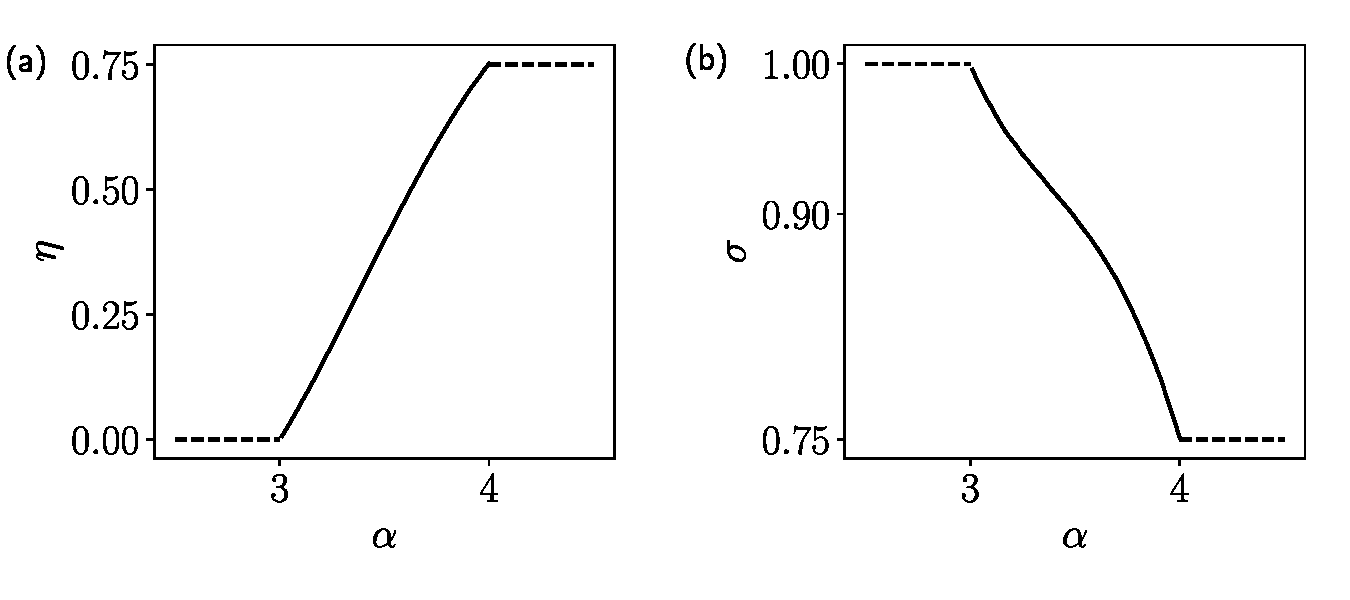
\includegraphics[width=0.9\textwidth]{Chapitre2/Figures/eta_kay.pdf}
	\caption{Évolution de l'exposant de rugosité (a) et de l'exposant d'hyperuniformité (b) associé avec la portée d'interaction dans le cadre théorique LR-CDP. Ces résultats encore non publiés ont été produits par K. Wiese qui nous a octroyé une autorisation de représentation dans ce manuscrit.}
	\label{fig:predic_kay}
\end{figure}

\subparagraph{}Un calcul similaire peut être mené pour déterminer l'exposant dynamique $z$ dans ce cadre. La transition de dépiégeage étant connue pour ne faire intervenir que deux exposants critiques indépendants, ces prédictions permettent en fait la caractérisation complète de la criticalité associée. En principe, les prédictions analytiques sont donc en mesure de déterminer complètement le cadre théorique LR-CDP. Toutefois, ces calculs restent soumis à des approximations et leur validation ne peut donc venir que de mesures numériques sur des modèles associés.

\section{Motivations pour une caractérisation numérique}

\subparagraph{}Dans cette section, nous motivons un peu plus spécifiquement la caractérisation numérique du cadre théorique LR-CDP en deux dimensions.

\subsection{Motivation principale : un point manquant dans la littérature}

\subparagraph{}De nombreuses études se sont déjà intéressées à l'influence d'un transport à longue portée sur le comportement critique des transitions de phase absorbantes. Dans le cadre de la percolation dirigée, cette influence a notamment été caractérisée de manière exhaustive en 1D \cite{hinrichsen_model_1999, hinrichsen_non_equilibrium_2007} et en 2D \cite{dos_santos_crossover_2018} sur des modèles de particules. Dans le cadre de la percolation dirigée conservée, cadre d'intérêt pour ce travail, les seules études numériques caractérisant l'impact de ce type d'interactions à longue portée viennent de l'étude de la transition de dépiégeage. Cependant, cette dernière trouvant essentiellement des réalisations physiques en 1D avec le cas de la ligne élastique, ces études se sont concentrées jusque là uniquement sur le cas unidimensionnel \cite{le_priol_long_range_2020, tanguy_individual_1998, rosso_roughness_2002, ramanathan_onset_1998}.

\subparagraph{}Dans ces travaux, les résultats numériques restent fidèles aux prédictions théoriques et confirment une évolution continue des exposants dans une gamme de portées déterminable par une analyse d'échelle. Toutefois, aucune étude à notre connaissance n'a été réalisée dans le cas d'un système appartenant à la classe CDP en 2D. Il manque alors à cette littérature un point de comparaison essentiel à notre étude dans les chapitres suivants. Par ailleurs cette caractérisation peut s'avérer utile en soi, simplement pour tester les prédictions analytiques présentées précédemment \cite{le_doussal_two_loop_2002}.

\subsection[Motivation secondaire : un cadre d'intérêt pour la modélisation de\\ systèmes réels]{Motivation secondaire : un cadre d'intérêt pour la modélisation de systèmes réels}

\subparagraph{}Bien que cela constitue notre motivation principale, la caractérisation de l'impact du transport à longue portée sur les systèmes de la classe CDP en 2D n'a pas seulement un intérêt théorique. En effet, certains modèles ou même certaines réalisations physiques correspondent vraisemblablement à cette situation. Cette étude peut alors permettre l'appréhension de leur criticalité plus spécifiquement.

\subparagraph{}Les réalisations physiques les plus évidentes de ce cadre sont celles associées à la transition de dépiégeage, de laquelle nous pouvons tirer deux exemples. Le premier est le mouvement de l'interface d'un fluide dans un milieu poreux par action de la gravité \cite{zhao_interface_2013}. Dans ce cas, le mouvement de l'interface bidimensionnelle peut être sujet à des interactions à longue portée permises par le fluide en volume. Le second concerne le mouvement des parois des domaines magnétiques dans les milieux magnétiques tridimensionnels \cite{alava_disorder_induced_1996}. Dans ce cas, ce sont les interactions entre charges magnétiques qui induisent la longue portée\cite{le_priol_long_range_2020}.

\subparagraph{}Un autre type de réalisations envisageables concerne les modèles épidémiques. Ces modèles que nous avons déjà introduit comme présentant une transition de phase absorbante ont de bonnes raisons de faire intervenir un transport à longue portée. En effet, dans ce cadre, celui-ci représente la capacité des vecteurs, i.e. des personnes, à se déplacer : par exemple une personne infectée prenant le train est susceptible de contaminer une autre personne à des centaines de kilomètres. La plupart des modèles épidémiologiques sont plutôt enclins à appartenir à la classe DP \cite{sanhedrai_epidemics_2022}. C'est notamment le cas du modèle SIS bien connu \cite{mota_critical_2018}. Toutefois, certains modèles plus complexes, faisant intervenir une diffusion locale des agents, peuvent présenter une criticalité différente, et dans une certaine limite, celle de la classe CDP \cite{nettuno_role_2024}. Dans ce cas, l'ajout d'un transport à longue portée pourrait donc effectivement être compris dans le cadre LR-CDP.

\subparagraph{}L'avantage du principe d'universalité est que, pour caractériser le comportement de tous ces systèmes, il suffit d'en caractériser un seul appartenant à la même classe. En étudiant un modèle numérique appartenant au cadre théorique LR-CDP en 2D, nous proposons une caractérisation de tous ces autres systèmes hypothétiques appartenant à la même classe. Ainsi, si l'intérêt principal de cette caractérisation numérique reste de constituer une base de comparaison pour l'étude des transitions de réversibilité et d'écoulement, elle trouve aussi un intérêt dans la modélisation de systèmes réels.

\section{Modèles}

\subparagraph{}Pour étudier l'influence du transport à longue portée dans la classe CDP en 2D, nous nous concentrons sur deux modèles emblématiques déjà présentés à la \autoref{sec:modelesCDP} : le modèle Manna et le ROM. Dans cette section, nous présentons l'implémentation numérique de ces deux modèles et leur généralisation par l'ajout d'un transport à longue portée. Cette généralisation nous permettra alors d'étudier le comportement critique de ces modèles numériques à n'importe quelle portée de transport pour ainsi confronter et compléter la théorie LR-CDP en 2D.

\subsection{LR-Manna}

\label{sec:ImplementationManna}

\subsubsection{Implémentation générale}

\subparagraph{}Nous commençons par présenter notre implémentation du modèle Manna. Le modèle Manna est un modèle très simple, appelant de ce fait une implémentation facilitée. Dans nos simulations, nous considérons un réseau 2D bipériodique de $N=L\times L$ sites, chacun indexé par un entier $i$, et positionné autour d'une position $\mathbf{r}_i = na\hat{\mathbf{e}}_x + ma \hat{\mathbf{e}}_y$ avec $(n,m) \in \mathbb{Z}^2$. $a$ représente le pas du réseau. Sur l'ensemble de ces $N$ sites sont disposés initialement et de manière aléatoire $N_p$ particules.

\subparagraph{}\`A chaque pas de temps $t_i$ de la dynamique, les $n$ sites accueillant plus de $m$ particules sont considérés comme actifs. Ceux-ci redistribuent alors l'entièreté de leur masse (i.e. leurs particules) aux sites directement voisins, et ce de manière aléatoire. La redistribution de masse de tous les sites actifs se fait de manière synchrone, i.e. sur le même pas de temps. \`A la fin de cette redistribution, un nouveau pas de temps est initié.

\subparagraph{}L'activité du système au pas de temps $t_i$ est alors donnée par la proportion de sites actifs $A(t_i) = n(t_i)/N$. Par ailleurs, la densité de particules $\phi$ correspond simplement au rapport $\phi = N_p/N$ et peut donc prendre des valeurs plus ou moins grandes en fonction du seuil $m$ choisi. Ce modèle présente alors une transition de phase absorbante séparant une phase active où l'activité $A$ prend une valeur moyenne finie à temps long pour $\phi>\phi_c$, d'une phase absorbante où le système finit par tomber dans un état absorbant pour $\phi<\phi_c$. La valeur de la densité critique du système $\phi_c$ dépend des détails microscopiques d'implémentation choisis. Elle ne peut donc pas a priori être reprise de travaux précédents. 

\subsubsection{Transport à longue portée}

\subparagraph{}Dans le modèle Manna original, les particules sur les sites actifs font des sauts à courte portée. L’extension de cette dynamique au transport à longue portée y prend donc une forme évidente. Dans ce cas, les particules redistribuées ne le sont plus uniquement sur les sites voisins mais, à la place, celles-ci font des sauts $\mathbf{r}$ largement distribués selon :

\begin{equation}
	P(\mathbf{r}) \sim \frac{1}{r^\alpha}.
\end{equation}

\noindent Dans un espace de dimension $D$, cela revient donc à effectuer des sauts de taille $\Delta = |\mathbf{r}|$ distribuée selon :

\begin{equation}
	P_\Delta(\Delta) \sim \frac{1}{\Delta^{1+\alpha-D}}.
	\label{eq:sauts}
\end{equation}

\subparagraph{}Pour chaque particule sur un site actif, nous générons donc un nombre aléatoire $\Delta$ distribué de la sorte. Nous générons ensuite une direction aléatoire $\theta$ permettant de définir le déplacement $\Delta_x = \Delta \cos \theta$ selon $\hat{\mathbf{e}}_x$ et $\Delta_y = \Delta \sin \theta$ selon $\hat{\mathbf{e}}_y$. Les deux réels $\Delta_x$ et $\Delta_y$ sont alors convertis en entiers pour représenter une distance en nombre de sites. Enfin, les conditions aux limites périodiques sont appliquées pour déterminer le site d'arrivée de la particule. La procédure complète est résumée sur la \autoref{fig:LRModels}-(a).

\begin{figure}[h]
	\centering
	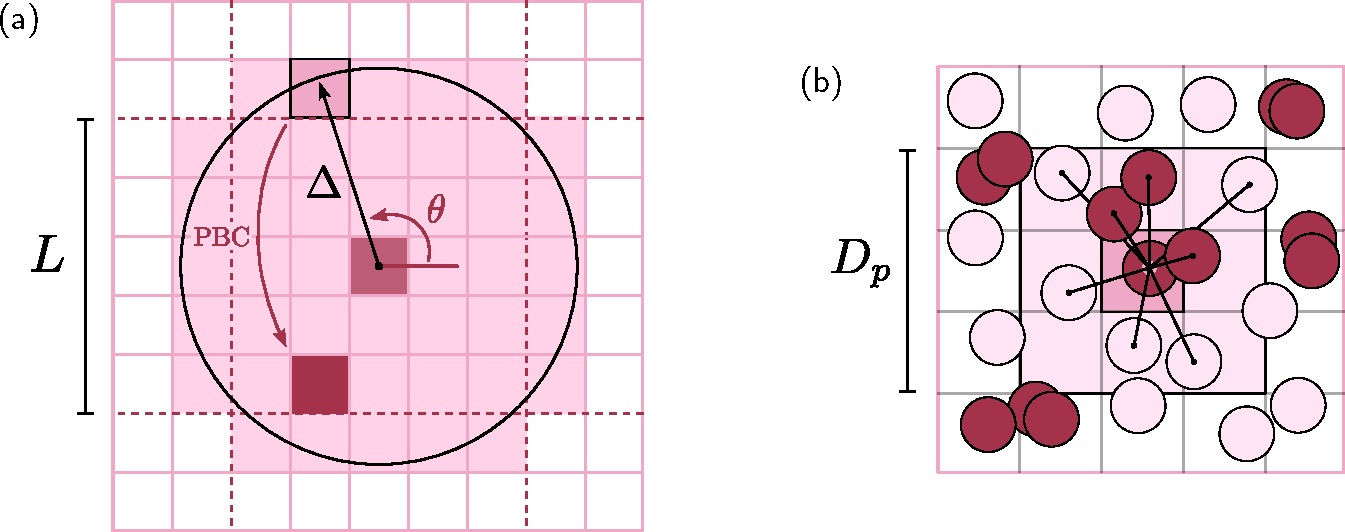
\includegraphics[width=\textwidth]{Chapitre2/Figures/Modeles/MannaJumps.pdf}
	\caption{Implémentation numérique des modèles LR-Manna et LR-ROM. (a) Procédure de saut à longue portée dans le modèle LR-Manna. PBC signifie \textit{periodic boundary conditions}. (b) Méthode cell-list pour la détermination des recouvrements dans le LR-ROM. En 2D, seules 9 cellules ont besoin d'être sondées pour déterminer les contacts d'une particules.}
	\label{fig:LRModels}
\end{figure}

\subparagraph{}Par cette implémentation numérique, il est possible d'étudier la transition de phase absorbante associée au modèle pour chaque portée $\alpha$. Dans la suite, nous appelons ce modèle généralisé LR-Manna.

\subsection{LR-ROM}

\label{sec:implementation_ROM}

\subsubsection{Implémentation générale}

\subparagraph{}Le second modèle que nous utilisons pour notre caractérisation numérique est le ROM. Ce modèle étant très proche du modèle Manna, son implémentation est très similaire. La différence principale qui les sépare vient du fait que la dynamique des particules a lieu dans ce cas en espace continu (par opposition au réseau de sites du modèle Manna). 

\subparagraph{}Pour son implémentation, $N_p$ particules de diamètre $D_p$ sont disposées initialement aléatoirement sur un espace 2D bipériodique de volume $L\times L$. Au début de chaque pas de temps $t_i$, les particules se recouvrant avec une autre particule sont considérées comme actives. Chaque particule active effectue alors un déplacement de manière synchrone décomposé en deux déplacements aléatoires $\Delta_x$ et $\Delta_y$, chacun de taille typique $a_p$. \`A l'issue de ce déplacement, un nouveau pas de temps est initié.

\subparagraph{}L'activité dans le ROM est définie comme la proportion de particules actives à un pas de temps donné et la densité $\phi$ comme la fraction d'espace occupée par les particules. Celles-ci étant choisies sphériques, nous avons $\phi = \frac{\pi D_p^2 N_p}{4 L^2}$ en 2D. De la même façon que le modèle Manna, le ROM ainsi défini présente une transition de phase absorbante de paramètre d'ordre $\phi$.

\subsubsection{Transport à longue portée}

\subparagraph{}Pour implémenter le transport à longue portée dans le ROM, nous utilisons exactement la même méthode que dans le cas du modèle Manna : à la place de faire des sauts finis de taille typique $a_p$, les particules actives font des sauts de taille $\Delta$ largement distribuée selon l'\autoref{eq:sauts}. Dans ce cas, nous nommerons cette généralisation du modèle LR-ROM.

\subsection{Détails d'implémentation}

\label{sec:DetImpl}

\subsubsection{Distributions de sauts}

\subparagraph{}Pour générer les sauts à longue portée dans les deux modèles, nous utilisons une méthode d'inversion \cite{devroye_general_1986} permettant générer des nombres aléatoires distribués selon :

\begin{equation}
	P_\Delta(\Delta) \sim \left\{
	\begin{aligned}
	& \Delta^{D-\alpha-1},\quad \text{si } \Delta > a, D_p\\
	& 0, \quad \text{sinon}
	\end{aligned}\right.
\end{equation}

\noindent le cut-off à petits $\Delta$ étant nécessaire à l'intégrabilité de la distribution pour $\alpha > D$. En pratique, nous commençons par tirer un nombre réel $x$ uniformément distribué dans $[0,1[$ grâce à des algorithmes pré-existants, puis $\Delta$ est obtenu par la transformation :

\begin{equation}
	\Delta = (1-x)^\frac{1}{D-\alpha}.
\end{equation}

\subsubsection{Méthode cell-list dans le ROM}

\subparagraph{}Dans le ROM et le LR-ROM, la condition de recouvrement entre une particule située en $\mathbf{r}$ et une particule située en $\mathbf{r}^\prime$ correspond à $|\mathbf{r}-\mathbf{r}^\prime|<D_p$. Afin de déterminer si une particule est active au début d'un pas de temps, il est donc nécessaire de calculer sa distance à toutes les autres particules du système. En principe, ce calcul de distance admet une complexité d'ordre $N_p^2$, ce qui rend la recherche de recouvrement fastidieuse. Pour remédier à ce problème, nous utilisons une méthode dite cell-list \cite{allen_computer_2017} dont le principe est résumé à la \autoref{fig:LRModels}-(b).

\subparagraph{}Le principe de cette méthode est de découper l'espace de volume $L\times L$ en une collection de $ n \times n $ cellules de dimension $\frac{L}{n}\times \frac{L}{n}$. \`A chaque pas de temps, nous identifions à quelle cellule $i$ appartient chacune des $N_p$ particules. La portée de l'interaction de contact étant bornée par $D_p$, en choisissant $\frac{L}{n}=D_p$, seules les particules situées dans une cellule voisine\footnote{Ici la notion de voisinage prend en compte les conditions aux limites périodiques.} de la cellule $i$ sont susceptibles de recouvrir les particules situées dans la cellule $i$. Ainsi, cela restreint le calcul de distance à un sous-ensemble du système, diminuant alors la complexité de l'opération à l'ordre $N_p$.

\subsubsection{Parallélisation et implémentation GPU}

\subparagraph{}Les schémas numériques associés aux deux modèles sont relativement parallélisables. En effet, lors d'un pas de temps la mise à jour de la position des particules se fait de manière synchrone. De plus, lors de ce déplacement, aucun échange d'information n'est nécessaire entre les différents agents du système. Seules les conditions d'activité (recouvrement dans le ROM ou dépassement du seuil sur un site dans le modèle Manna), qui n'ont lieu qu'une fois par pas de temps, nécessitent un partage de la mémoire. 

\subparagraph{}Afin d'en tirer parti, nous implémentons donc ces deux modèles via le langage CUDA \cite{cuda} afin de réaliser les simulations sur GPU (cartes graphiques). Par opposition aux CPU, les GPU sont dotées d'un bien plus grand nombre de cœurs, permettant ainsi un plus grand nombre d'opérations simultanées. Ces cœurs sont individuellement moins performants mais les opérations nécessaires à la réalisation de la dynamique Manna ou ROM sont très peu onéreuses et donc particulièrement adaptées à ce type d'architecture.

\subsubsection{Valeurs des paramètres}

\subparagraph{}Dans le ROM, nous prendrons comme unité de longueur du système le diamètre des particules et considérerons donc $D_p=1$. Dans le cas de sauts à courte portée, nous prendrons $a_p=1$.

\subparagraph{}Dans le modèle Manna, nous prendrons comme unité de longueur du système le pas du réseau et donc $a=1$.

\section{Méthodes de caractérisation du comportement critique}

\label{sec:methodchap2}

\subparagraph{}La caractérisation du comportement critique d'un système ou d'une classe d'universalité passe par la détermination de ses exposants. Dans cette section, nous présentons les méthodes utilisées pour la détermination spécifique des exposants critiques $\beta$ et $\gamma^\prime$, de l'exposant dynamique $\delta$ et de l'exposant d'hyperuniformité $\sigma$, tous présentés au \autoref{chapter:introduction}. Ces méthodes nous permettront de caractériser les transitions dans le LR-ROM et le modèle LR-Manna pour chaque portée $\alpha$ et seront ensuite réutilisées dans les chapitres suivants. De ce fait, nous nous attachons à les décrire de manière suffisamment précise.

\subsection{Détermination des exposants critiques}

\label{sec:MethodesExposants}

\subsubsection{Détermination du point critique}

\subparagraph{}La première étape essentielle à la caractérisation d'une transition de phase est la localisation de son point critique. Ici, cela correspond à la détermination de la densité critique $\phi_c$. Pour la mettre en œuvre, nous nous appuyons sur la loi d'évolution du paramètre d'ordre dans le régime critique :

\begin{equation}
	\langle A \rangle \sim \delta\phi^\beta, \quad \delta\phi = \frac{\phi-\phi_c}{\phi_c}.
\end{equation}

\noindent D'après celle-ci, la fonction $\langle A \rangle = f(\delta\phi)$ correspond à une droite de pente $\beta$ dans une représentation logarithmique. Cela peut donc représenter une méthode graphique pour la détermination de $\phi_c$ : la valeur recherchée est celle définissant la distance $\delta\phi$ permettant d'obtenir la courbe la plus proche d'une droite à petits $\delta\phi$. Si nous sous-estimons $\phi_c$, alors cette fonction montrera une courbure concave en échelle logarithmique. \`A l'inverse, si nous sur-estimons $\phi_c$, celle-ci montrera une courbure convexe. De cette manière, il est possible d'encadrer graphiquement la valeur adéquate de $\phi_c$ comme illustré à la \autoref{fig:PhicDeter}-(a). En pratique, afin de mieux percevoir les variations de forme de la courbe, nous examinons aussi l'évolution compensée $\langle A \rangle/\delta\phi^{\beta_t} = g(\delta\phi)$ par l'évolution attendue avec un exposant test $\beta_t$ en échelle log-lin (voir \autoref{fig:PhicDeter}-(b)). La méthode graphique d'encadrement associée est alors plus précise. Celle-ci permet donc de définir la densité critique $\phi_c$ et l'exposant $\beta$ comme les deux paramètres permettant d'obtenir une courbe constante à petits $\delta\phi$.

\begin{figure}[h]
	\centering
	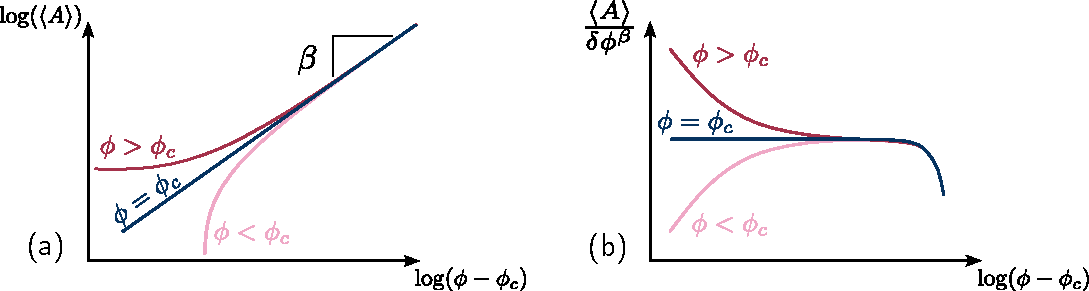
\includegraphics[width=\textwidth]{Chapitre2/Figures/Methodes/Phic.pdf}
	\caption{Méthode de détermination de la densité critique (a) en échelle logarithmique et (b) en échelle log-lin via une représentation compensée.}
	\label{fig:PhicDeter}
\end{figure}

\subparagraph{}Cette mesure repose donc finalement sur la détermination de la courbe $\langle A \rangle = f(\delta\phi)$ et donc sur les mesures précises de $\langle A \rangle$ pour différentes densités $\phi$. Pour réaliser ces mesures, à une taille $L$ de système donnée, nous laissons le système relaxer vers l'état stationnaire dans lequel nous mesurons la valeur moyenne de la variable instantanée $A(t)$. La détermination du régime stationnaire est effectuée graphiquement en représentant $A(t)$ en échelle logarithmique (voir \autoref{fig:DeltaDeter}). Afin de déterminer $\phi_c$, nous devons sonder le comportement du système proche du point critique et donc proche de la phase absorbante. Le problème est que, dans un système fini de taille $L$, les fluctuations de la dynamique peuvent amener le système dans un état absorbant même pour $\phi \gtrsim \phi_c$, rendant alors la détermination de $\langle A \rangle$ impossible. Les fluctuations critiques diminuant avec la taille du système $L$, il est possible de contourner cet obstacle en considérant des systèmes plus grands. La méthode que l'on choisit consiste alors à augmenter la taille $L$ du système à mesure que l'on considère des densités $\phi$ plus proches de $\phi_c$ afin de ne jamais risquer de tomber dans un état absorbant. In fine, la courbe $\langle A \rangle = f(\delta\phi)$ obtenue correspond donc  à une concaténation de courbes obtenues pour différentes tailles $L$ du système.

\subparagraph{}Ne pas se concentrer uniquement sur la plus grande taille $L$ envisageable est un choix permettant de réduire l'effort numérique associé. En effet, plus un système est grand, plus la simulation de sa dynamique est longue. Cette méthode suppose cependant que toutes ces courbes sont bien équivalentes, i.e. que $\phi_c$ est indépendant de $L$. En théorie, la valeur estimée de $\phi_c$ sur un système de taille $L$ présente toujours une dépendance de taille finie, mais dans notre cas il est possible de s'en affranchir raisonnablement. En effet, statistiquement, si un système tombe dans l'état absorbant c'est parce que la longueur de corrélation $\xi$ de la dynamique associée est devenue au moins comparable à la taille $L$ de ce système. Or, par définition des effets de taille finie, la dépendance de $\phi_c$ en $L$ n'est visible que lorsque la dynamique "ressent" la taille du système, i.e. $\xi \gtrsim L$. Ainsi, en ne sondant que les états statistiquement non absorbés, nous pouvons considérer que $\phi_c$ est indépendant de $L$. Cette hypothèse se confirme alors très bien avec nos mesures puisque celles faites à différentes tailles de système se recouvrent parfaitement, comme représenté sur la \autoref{fig:Effet_Taille_Phic} dans le cas du modèle Manna. Toutefois, cela invite à ne pas sonder le système trop proche de sa limite d'absorption et de préférer systématiquement le passage à une taille supérieure.

\begin{figure}[h]
	\centering
	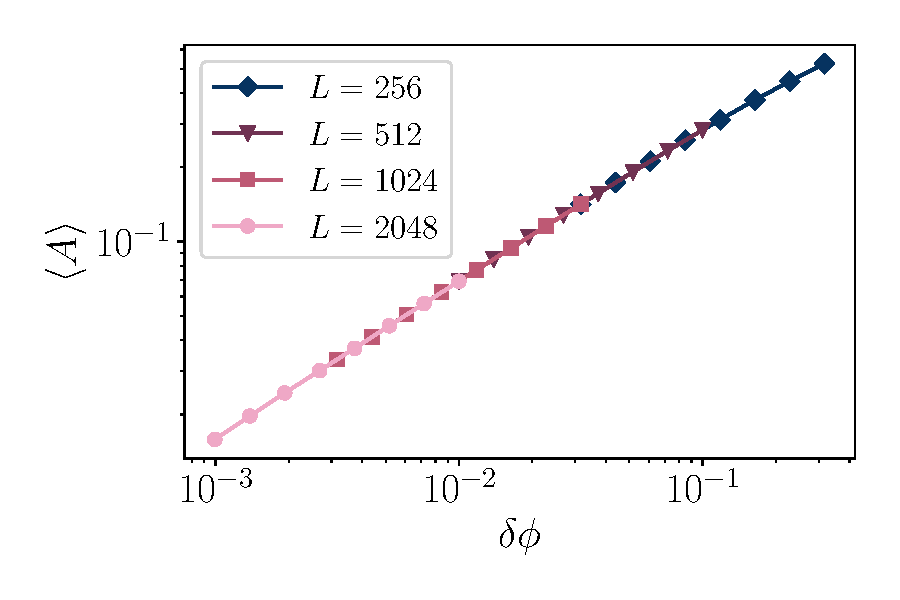
\includegraphics[width=0.6\textwidth]{Chapitre2/Figures/Phi_cindep.pdf}
	\caption{Détermination de la courbe $\langle A \rangle = f(\delta\phi)$ dans le ROM. La superposition des courbes pour différentes tailles de système dans leur domaine de non-absorption valide l'approche considérant $\phi_c$ indépendante de $L$. Ici, on a $\phi_c \approx 0.23520$}
	\label{fig:Effet_Taille_Phic}
\end{figure}

\subsubsection{Détermination des exposants statiques}

\subparagraph{}Une fois la densité critique $\phi_c$ déterminée précisément pour un système, il est possible de mesurer les exposants critiques de la transition. L'exposant statique $\beta$ est en fait déjà déterminé lors de la détermination de $\phi_c$ via les méthodes graphiques présentées précédemment. Afin d'obtenir un ordre de grandeur de son incertitude, nous effectuons un ajustement de la courbe $\langle A \rangle = f(\delta\phi)$ à petits $\delta\phi$ en échelle logarithmique pour les deux valeurs extrémales de l'encadrement de $\phi_c$.

\subparagraph{}Pour déterminer l'exposant des fluctuations critiques $\gamma^\prime$, nous mesurons les fluctuations de l'activité $\langle \delta A^2\rangle = L^D\times(\langle A ^2 \rangle - \langle A \rangle^2)$ dans l'état stationnaire sur les mêmes courbes $A(t)$ qui ont permis de mesurer $\langle A \rangle$. La densité critique ayant été précédemment déterminée, nous déterminons $\gamma^\prime$ directement par ajustement de la courbe $\langle \delta A^2\rangle = g(\delta\phi)$ en échelle logarithmique. La variance correspondant à un moment d'ordre supérieur par rapport à la moyenne, sa détermination précise est plus délicate. Ainsi, la détermination de $\gamma^\prime$ sera généralement entachée de plus grandes erreurs. Toutefois, étant donné que nous nous concentrerons essentiellement sur l'évolution de $\gamma^\prime$ avec la portée dans la suite de ce travail, nous nous satisferons d'une telle précision. Les incertitudes sur cette détermination sont associées à l'incertitude sur l'ajustement de la courbe en échelle logarithmique\footnote{En pratique, nous constatons que les incertitudes sur $\gamma^\prime$ liées à la détermination de $\phi_c$ (et donc la définition de $\delta\phi$) sont négligeables devant l'incertitude de l'ajustement effectué à une valeur de $\phi_c$ donnée.}.

\subsubsection{Détermination de l'exposant dynamique}

\subparagraph{}Comme nous l'avons vu au \autoref{chapter:introduction}, en partant d'une configuration initiale aléatoire, proche du point critique, le système relaxe vers l'état stationnaire de manière algébrique :

\begin{equation}
	A(t) \sim t^{-\delta}.
	\label{eq:deltaJumps}
\end{equation}

\noindent L'exposant $\delta$ ainsi défini permet de caractériser la transition d'un point de vue dynamique. Une difficulté liée à sa détermination est que le régime de temps dans lequel le comportement de l'\autoref{eq:deltaJumps} est valable est situé entre un comportement non-universel à temps courts et une saturation à temps long du fait que $\phi>\phi_c$. Il n'est donc pas aisé de mesurer $\delta$ par un simple ajustement sur une unique courbe. 

\subparagraph{}Pour remédier à ce problème, nous utilisons une méthode de redimensionnement comme outil de détermination plus précis. Pour ce faire, nous nous appuyons sur le fait que, hors du régime de temps courts, l'activité dans le système prend la forme :

\begin{equation}
	A(t, \delta\phi) \sim \langle A \rangle (\delta\phi) + t^{-\delta} \sim \delta\phi^\beta + t^{-\delta} \Rightarrow \frac{A(t)}{\delta\phi^\beta} \sim 1 + \left(\frac{t}{\delta\phi^{-\beta/\delta}}\right)^{-\delta},
\end{equation}

\noindent par définition de l'exposant $\beta$. Ainsi, si nous redimensionnons $A(t)$ par $\delta\phi^\beta$ et $t$ par $\delta\phi^{-\beta/\delta}$, nous obtenons une évolution indépendante de la distance au point critique $\delta\phi$. En d'autres termes, si l'on mesure l'évolution $\frac{A(t)}{\delta\phi^\beta} = f \left(\frac{t}{\delta\phi^{-\beta/\delta}} \right)$ pour différentes densités $\phi$, les différentes évolutions se superposent graphiquement (voir \autoref{fig:DeltaDeter}). $\beta$ et $\phi_c$ étant précédemment mesurés, $\delta$ est alors déterminé comme l'exposant qui permet la superposition de toutes les courbes sur une courbe maîtresse sous ce redimensionnement. L'incertitude de mesure sur cet exposant est alors donnée par la gamme d'exposants pour laquelle la superposition des courbes est jugée satisfaisante. Ce principe de mesure par redimensionnement s'avère très efficace, et sera utilisé à plusieurs reprises dans les chapitres suivants pour mesurer d'autres quantités.

\begin{figure}[h]
	\centering
	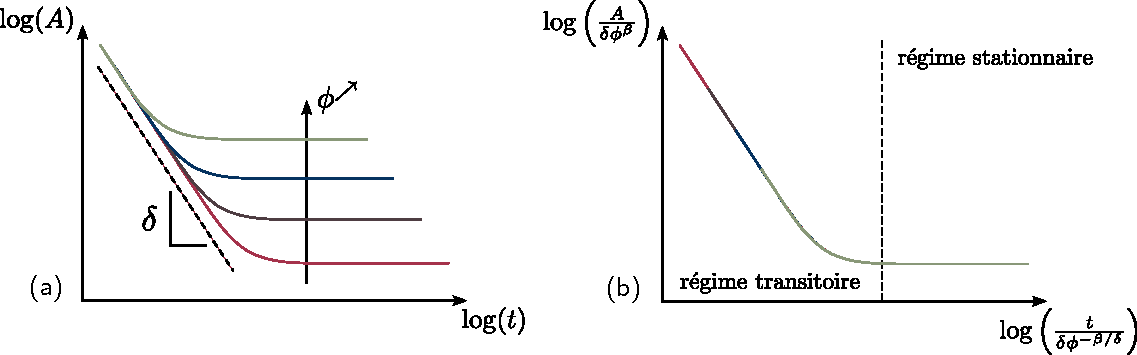
\includegraphics[width=\textwidth]{Chapitre2/Figures/Methodes/Delta.pdf}
	\caption{Méthode de détermination de l'exposant dynamique $\delta$. (a) Évolution de l'activité dans le système en fonction du temps pour différentes densités $\phi$. (b) Redimensionnement du temps et de l'activité par la distance au point critique permettant la superposition des différentes courbes sur une courbe maîtresse.}
	\label{fig:DeltaDeter}
\end{figure}

\subsection{Caractérisation de l'hyperuniformité}

\label{sec:MethodHU}

\subparagraph{}Dans cette dernière sous-section nous présentons les méthodes utilisées pour sonder les propriétés d'hyperuniformité dans nos modèles. Celles-ci reposant sur des propriétés de structure, nous ne pouvons pas nous limiter à une étude du comportement macroscopique pour déterminer l'exposant $\sigma$. Toutefois, la philosophie des mesures utilisées en pratique restent très similaires.

\subsubsection{Mesure directe du facteur de structure}

\subparagraph{}Comme nous l'avons évoqué au \autoref{chapter:introduction}, les systèmes appartenant à la classe CDP présentent des propriétés hyperuniformes. Proche de la transition, la répartition des particules dans l'espace présente des corrélations à longue portée. Une manière de les caractériser  est de passer dans l'espace réciproque. En effet, dans de tels systèmes, cette propriété se traduit par une diminution du facteur de structure $S(\mathbf{q})$ à petits $q$ selon :

\begin{equation}
	S(\mathbf{q})\sim q^{\alpha_\text{HU}}, \quad 0 < \alpha_\text{HU} < 1.
\end{equation}

\noindent L'exposant $\alpha_\text{HU}$ permet alors de caractériser la transition de phase au même titre qu'un autre exposant critique. Le cas limite $\alpha_\text{HU}$ = 0 représente une répartition totalement décorrélée à grande échelle.

\subparagraph{}Une manière de quantifier l'hyperuniformité caractéristique d'un comportement critique est donc de mesurer précisément le facteur de structure à petits $q$ dans un état stationnaire proche du point critique afin d'en déduire une estimation de cet exposant $\alpha_\text{HU}$.

\subsubsection{Méthode de box-counting}

\paragraph{Définition}

\subparagraph{}Une autre façon de procéder est de revenir à la définition initiale de l'hyperuniformité \cite{torquato_local_2003}. Comme nous l'avons présenté à la \autoref{sec:introHU}, dans un système hyperuniforme, la variance $\langle \delta n^2\rangle_l$ du nombre de particules contenues dans un sous-ensemble du système de volume $l^D$ se comporte comme :

\begin{equation}
	\langle \delta n^2\rangle_l \sim \langle n \rangle_l^\sigma , \quad  \sigma < 1,
	\label{eq:HUBC}
\end{equation}

\noindent $\sigma = 1$ représentant le cas trivial de l'absence de corrélations. Cette représentation de l'hyperuniformité est en fait directement liée à celle observée dans l'espace réciproque, les exposants $\sigma$ et $\alpha_\text{HU}$ étant reliés par la relation \cite{torquato_local_2003, lei_non_equilibrium_2024, hexner_hyperuniformity_2015} :

\begin{equation}
	\sigma = \left\{
	\begin{aligned}
	&1-\frac{\alpha_\text{HU}}{D}, \quad\text{si } 0 < \alpha_\text{HU} < 1 \\
	&1-\frac{1}{D}, \quad \text{si } \alpha_\text{HU} > 1
	\end{aligned}
	\right.
	\label{eq:eqsigmaalphahu}
\end{equation}

\subparagraph{}Une méthode de qualification de l'hyperuniformité, que nous appelons méthode box-counting, consiste donc à mesurer $\langle \delta n^2\rangle_l$ et pour différentes tailles $l$ de sous-ensembles dans des configurations de l'état stationnaire du système proche de son point critique. Ainsi, nous pouvons étudier son évolution en fonction de $\langle n \rangle_l$ pour déterminer directement l'exposant $\sigma$ associé.

\subparagraph{}Si la définition de l'hyperuniformité s'est construite autour de l'\autoref{eq:HUBC}, plusieurs travaux s'intéressent aux fluctuations de densité locale $\langle \delta \rho^2\rangle_l$ au lieu du nombre de particules, et en fonction de l'extension $l$ du sous-ensemble au lieu du nombre moyen de particules \cite{hexner_hyperuniformity_2015, bub_lee_hyperuniformity_2019}. Dans ce cas, on définit la loi d'échelle entre ces quantités par l'exposant $\lambda$ selon :

\begin{equation}
	\langle \delta \rho^2\rangle_l \sim l^{-\lambda},
\end{equation}

\noindent qui est alors directement relié à l'exposant $\sigma$ par :

\begin{equation}
	\sigma = 2 - \frac{\lambda}{D}.
\end{equation}

\paragraph{Implémentation}

\subparagraph{}Dans ce chapitre, nous caractérisons l'hyperuniformité des modèles de sauts à longue portée via la méthode de box-counting. Pour ce faire, nous générons des configurations par la dynamique stationnaire de systèmes proches du point critique. Chacune de ces configurations est alors analysée de la même façon.

\subparagraph{}Pour le modèle Manna comme pour le ROM, nous découpons l'espace carré de surface $L\times L$ en une collection compacte de sous-ensembles carrés de taille $l\times l$. En comptant le nombre de particules présentes dans chacun de ces sous-ensembles, nous en déduisons la variance $\langle \delta n^2\rangle_l$ associée. Le nombre moyen de particules dans les sous-ensembles est directement donné par  $\langle n \rangle_l= \phi \times l^D$. Si à petits $\langle n \rangle_l$ l'évolution est satisfaisante avec une mesure unique, celle à grande échelle nécessite un certain effort numérique. La première raison évidente est le manque d'échantillonnage aux grandes échelles dans les configurations de taille finie : plus $l$ est grand, moins il y a de sous-compartiments. La seconde raison est que les fluctuations à grande échelle sont associées à des temps de corrélation plus grands, ce qui implique une forte séparation temporelle entre deux configurations quasi-indépendantes dans l'état stationnaire. Afin d'obtenir une statistique raisonnable, chaque mesure associée à une densité $\phi$ et une portée $\alpha$ est donc moyennée dans le temps et sur différents états initiaux complètement décorrélés les uns des autres.

\paragraph{Détermination par redimensionnement}

\subparagraph{}En principe, la forme définie par l'\autoref{eq:HUBC} n'est valable qu'à des échelles de longueur $l$ suffisamment grandes, soit $\langle n \rangle_l \gg 1$. Pour mesurer l'exposant $\sigma$, il est donc nécessaire se placer à grande échelle. Par ailleurs, pour sonder un état stationnaire, il est aussi nécessaire se placer à une distance finie $\delta\phi>0$ du point critique, sans quoi le système tombera dans un état absorbant. Cette distance finie du point critique définit alors une échelle de longueur $l_c$, ou de manière équivalente un cut-off $\langle n \rangle_c$, au-delà de laquelle l'évolution algébrique n'est plus valide. En fait, dans nos mesures, au-delà de cette échelle de longueur, la courbe $\langle \delta n^2 \rangle = f(\langle n \rangle)$ présente un crossover non monotone vers l'évolution triviale $\sigma = 1$, aussi distinguable sur l'évolution du facteur de structure \cite{hexner_hyperuniformity_2015,hexner_noise_2017, hexner_enhanced_2017 }. En pratique, au-delà de $l_c$, avant que l'exposant effectif local de la courbe $\langle \delta n^2 \rangle = f(\langle n \rangle)$ ne rejoigne le cas décorrélé avec $\sigma_\text{eff}=1$, il diminue ($\sigma_\text{eff}<\sigma$). Cette diminution est visible sur les évolutions représentées à la \autoref{fig:HUCM} par exemple. L'évolution globale de $\langle \delta n^2 \rangle$ à grands $\langle n \rangle$ peut donc être modélisée par l'équation suivante :

\begin{equation}
	\langle \delta n^2 \rangle \sim \langle n \rangle^\sigma g\left( \frac{\langle n \rangle}{\langle n \rangle_c} \right),
\end{equation}

\noindent avec $g(x)$ constante pour $x\ll 1$ puis initialement décroissante pour $x>1$, définissant la forme du crossover.

\subparagraph{}Du fait de la présence de deux crossovers, un de petite taille et un dû à la distance finie au point critique, il peut s'avérer difficile de mesurer l'exposant $\sigma$ ou $\lambda$ sur une unique courbe. Une méthode utilisée dans \cite{hexner_hyperuniformity_2015} consiste alors à étudier différentes courbes associées à différentes distances du point critique $\delta\phi$. En supposant que l'échelle de longueur définissant le cut-off se comporte comme la longueur de corrélation $\xi\sim \delta\phi^{-\nu_\perp}$, nous avons $\langle n \rangle_c \sim \delta\phi^{-D\nu_\perp}$. Ainsi, en redimensionnant $\langle n \rangle$ par $ \delta\phi^{-D\nu_\perp}$ et $\langle \delta n^2 \rangle$ par $\delta\phi^{-\nu_\perp D \sigma}$, les courbes obtenues pour différentes densités devraient se superposer sur une même courbe maîtresse. Cela définit alors une potentielle méthode graphique pour la mesure de $\sigma$, utilisant les effets de crossover à son avantage. Néanmoins, en pratique, cette méthode peut s'avérer coûteuse numériquement car elle suppose la détermination précise d'un ensemble de courbes à différentes densités $\phi$. C'est pourquoi, nous ne l'utiliserons que dans le cas d'une analyse plus poussée.

\subsubsection{Des mesures complexes}

\subparagraph{}Si l'hyperuniformité n'a jamais été mesurée dans les modèles de transport à longue portée, celle-ci a fait l'objet de nombreuses études dans le cas de courte portée. Notamment, le ROM et le modèle Manna ont été caractérisés en ce sens à plusieurs reprises.

\subparagraph{}Les première études ont été menées par Hexner et Levine \cite{hexner_hyperuniformity_2015}, Tjhung et Berthier \cite{tjhung_hyperuniform_2015} et Weijs et al \cite{weijs_emergent_2015}. Dans \cite{tjhung_hyperuniform_2015}, les auteurs ont mesuré proche de la transition un exposant $\alpha_\text{HU} \approx 0.45$ dans le cas du ROM en 2D. En parallèle, l'étude \cite{hexner_hyperuniformity_2015} s'est concentrée sur les propriétés de différents modèles appartenant à la classe CDP, dont le modèle Manna et le ROM. Dans le cas bidimensionnel, il a été déterminé $\lambda\approx 2.45$ et $\alpha_\text{HU}\approx 0.45$, deux mesures cohérentes et indiquant $\sigma \approx 0.775$. Ces valeurs ont alors été confirmées dans \cite{weijs_emergent_2015} et comparées à une situation expérimentale. Par la suite, ces résultats furent retrouvés dans des généralisations de ces modèles \cite{hexner_noise_2017, ma_hyperuniformity_2019}.

\subparagraph{}Les résultats précédents confortent l'idée que les exposants d'hyperuniformité sont universels, i.e. communs à tous les modèles de la classe CDP. Toutefois, une étude plus récente semble mettre en défaut cette idée. Dans \cite{bub_lee_hyperuniformity_2019}, en utilisant des tailles de systèmes plus grandes que dans les études précédentes, les auteurs semblent relever une légère différence de l'ordre de 5\% entre les exposants d'hyperuniformité du ROM et du modèle Manna en 2D, qualifiant alors l'hyperuniformité de "faiblement universelle" dans ces modèles. Dans \cite{wiese_hyperuniformity_2024}, il a par ailleurs été montré que les mesures d'hyperuniformité peuvent être soumises à de forts effets de taille finie, affectant significativement les résultats des mesures. Sans nécessairement remettre en question l'universalité des propriétés hyperuniformes, ces études nous invitent donc à questionner nos méthodes et rester critiques face aux mesures que nous présenterons.

\section{Exposants critiques}

\subparagraph{}Afin de préciser quantitativement l'évolution des exposants critiques dans le cadre LR-CDP en 2D, nous nous concentrons d'abord sur sa représentation par le modèle LR-ROM. Dans cette section, nous présentons les résultats obtenus quant à la caractérisation des exposants critiques associés à chaque portée de transport $\alpha$.

\subparagraph{}Dans la \autoref{sec:LRCanonique} nous avons vu que dans ce cadre nous attendions une évolution continue de la criticalité entre $\alpha = 4$ et $\alpha=3$. Pour $\alpha\geq 4$ nous nous attendons à retrouver les valeurs des exposants reportées dans la première ligne du \autoref{tab:expocrit_LRROM}. Pour $\alpha\leq 3$, nous nous attendons à retrouver les valeurs triviales des exposants associés au champ moyen. Pour cerner et caractériser précisément la zone d'évolution continue des exposants, nous nous attachons par la suite à caractériser les portées de transport dictées par $\alpha \in \{ 6, 5, 4, 3.75, 3.5, 3.25, 3, 2.5  \}$.

\label{sec:expcritjumps}

\subsection{Exposants statiques}

\subparagraph{}En appliquant les méthodes décrites à la \autoref{sec:MethodesExposants}, nous déterminons les densités critiques $\phi_c$ des systèmes pour chacune des portées $\alpha$. Pour ce faire, nous utilisons des tailles de systèmes allant jusqu'à $L=16384$, correspondant à des nombres de particules allant jusqu'à $N\approx 6\times 10^7$. Un exemple de détermination est représenté à la \autoref{fig:DeterPhicJumps} dans le cas $\alpha = 3.75$. Les exposants $\beta$ et $\gamma^\prime$ et leurs incertitudes sont alors mesurés, leurs valeurs sont reportées dans le \autoref{tab:expocrit_LRROM} et leurs évolutions sont représentées sur la \autoref{fig:EvolExpJumps}.

\begin{figure}[h]
	\centering
	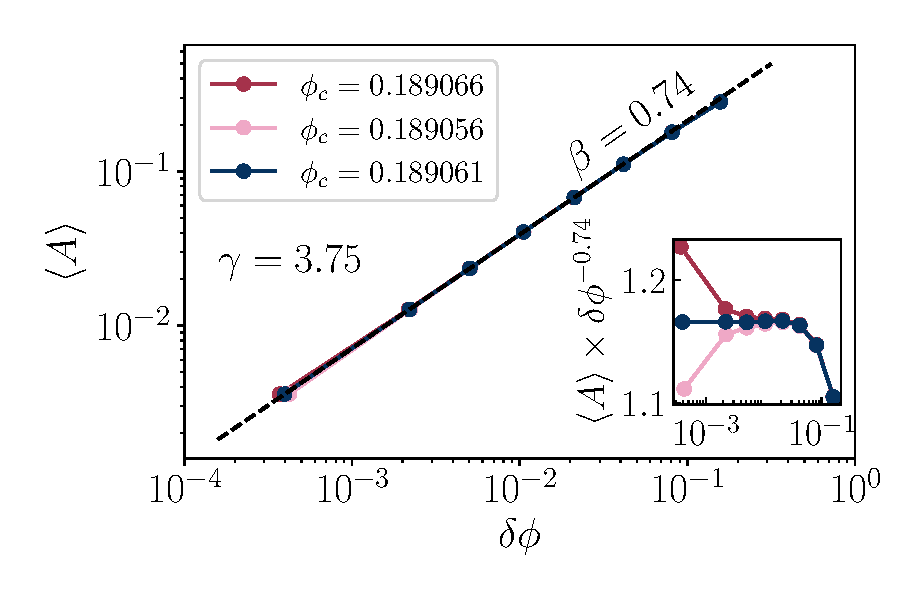
\includegraphics[width=0.7\textwidth]{Chapitre2/Figures/Exposants/Deter_phic_gamma375_LRROM.pdf}
	\caption{Détermination de la densité critique dans le LR-ROM pour $\alpha=3.75$. En encart, la représentation compensée permet de distinguer clairement $\phi_c = 0.189061$ comme une meilleure estimation que $\phi_c = 0.189056$ et $\phi_c = 0.189066$}
	\label{fig:DeterPhicJumps}
\end{figure}

\subparagraph{}Dans la limite de courte portée, nous retrouvons le comportement critique associé à la classe CDP. Pour $\alpha > 4$, nous mesurons $\beta\approx 0.63$ et $\gamma^\prime \approx 0.37$, tous deux en accord avec $\beta_\text{CDP}^{2D}\approx 0.64$ et $\gamma_\text{CDP}^{\prime 2D}\approx 0.37$. \`A l'opposé, dans la limite de longue portée, nous retrouvons les exposants associés au champ moyen de la classe CDP. Notamment, pour $\alpha = 2.5$, l'accord est exact dans la limite des incertitudes de détermination. L'évolution des exposants prend majoritairement place entre $\alpha = 4$ et $\alpha = 3$, en accord avec le cadre théorique. Toutefois, nous notons un léger écart avec les valeurs attendues au niveau de ces bornes. Notamment, pour $\alpha = 4$, nous mesurons $\beta \approx 0.69$ soit une valeur légèrement supérieure à celle associée à la courte portée. Nous discuterons de l'origine potentielle de cet écart dans la section suivante.

\subparagraph{}En pratique, la détermination de l'exposant $\nu_\perp$ nécessite l'analyse des corrélations spatiales d'activité dans le système afin d'en déduire la longueur de corrélation $\xi$ associée. Toutefois, il existe une relation d'échelle entre les exposants $\beta$, $\gamma^\prime$ et $\nu_\perp$, présentée au \autoref{chapter:introduction} :

\begin{equation}
	2\beta + \gamma^\prime = \nu_\perp D.
	\label{eq:HyperScaling}
\end{equation}

\noindent En supposant que celle-ci reste valable à n'importe quelle portée en-dessous de la dimension critique $D_c = 2(\alpha-D)$, nous pouvons tirer profit de cette relation pour dériver l'exposant $\nu_\perp$ associé. En utilisant les valeurs mesurées de $\beta$ et $\gamma^\prime$, nous répertorions dans le \autoref{tab:expocrit_LRROM} la valeur $\nu_\perp^*$ déduite de cette relation. Comme nous l'avons mentionné à la \autoref{sec:LRCanonique}, la subtilité est que, en présence d'interactions à longue portée, la valeur champ moyen de cet exposant est donnée par $\nu_\perp = 1/(\alpha-D)$, et donc dépendante de $\alpha$. En gardant cela en mémoire, nous observons de la même façon que les valeurs de $\nu_\perp^*$ suivent une évolution continue de la limite de courte portée avec $\nu_\perp \approx 0.82$ pour $\alpha>4$ à la limite de champ moyen avec $\nu_\perp\approx 1 = 1/(\alpha-D)$ pour $\alpha=3$. Pour $\alpha < 3$, nous avons $D>D_c$ et il n'est donc plus possible d'utiliser la relation d'échelle pour déterminer $\nu_\perp$. 

%\begin{figure}[h]
%	\centering
%	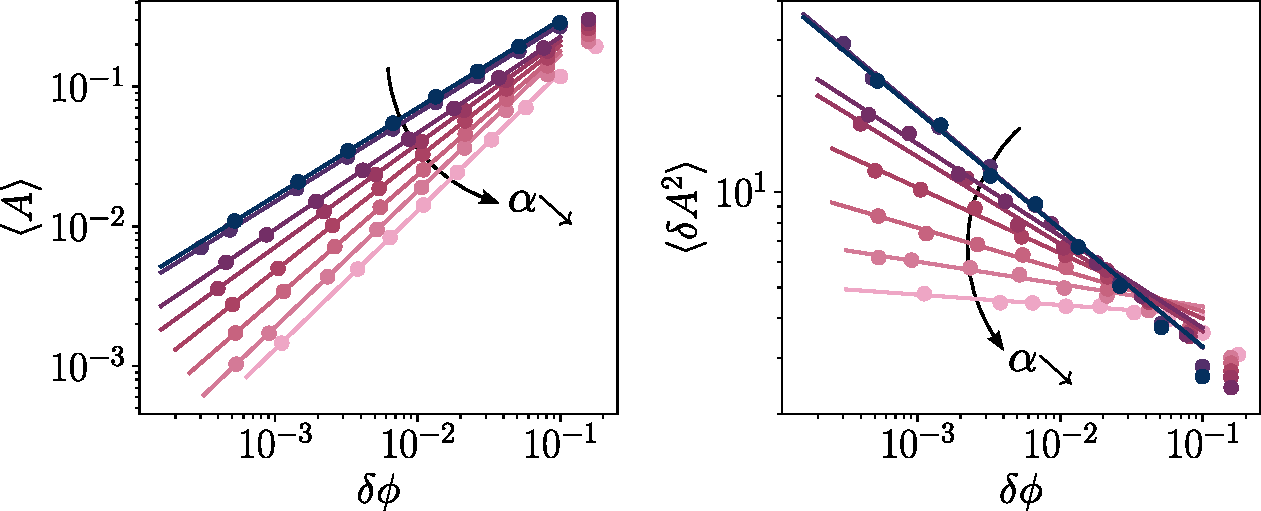
\includegraphics[width=\textwidth]{Chapitre2/Figures/Exposants/EvolMeanVar_Jumps.pdf}
%	\caption{}
%	\label{fig:EvolMeanVarJumps}
%\end{figure}

\subsection{Exposant dynamique}

\label{sec:expdynjump}

\subparagraph{}L'exposant dynamique $\delta$ est ensuite déterminé pour chaque portée $\alpha$ en suivant la méthode de redimensionnement précédemment présentée. Un exemple de détermination est présenté pour $\alpha = 4$ à la \autoref{fig:DeltaDeterJumps}. Les valeurs estimées de cet exposant sont reportées dans le \autoref{tab:expocrit_LRROM} et leur évolution est représentée à la \autoref{fig:EvolExpJumps}.

\begin{figure}[h]
	\centering
	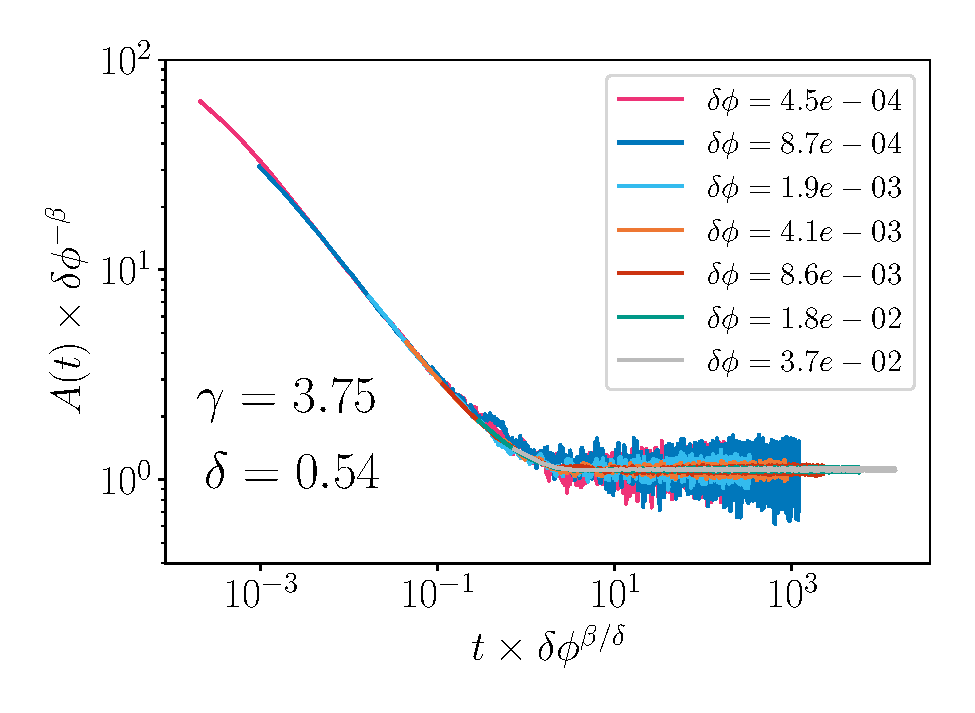
\includegraphics[width=0.7\textwidth]{Chapitre2/Figures/Exposants/DeltaDeter.pdf}
	\caption{Détermination de l'exposant dynamique $\delta$ par redimensionnement dans le LR-ROM pour $\alpha=3.75$.}
	\label{fig:DeltaDeterJumps}
\end{figure}

\subparagraph{}Comme dans le cas des exposants statiques, nous retrouvons les comportements limites de champ moyen $\delta_\text{CDP}^\text{CM}=1$ et de courte portée $\delta_\text{CDP}^{2D} \approx 0.42$ dans la limite des petits et des grands $\alpha$. De la même façon, l'évolution significative de l'exposant a lieu dans la gamme $3<\alpha<4$ bien que nous notions encore une fois un léger écart aux valeurs attendues au niveau de ces bornes.

\begin{figure}[h]
	\centering	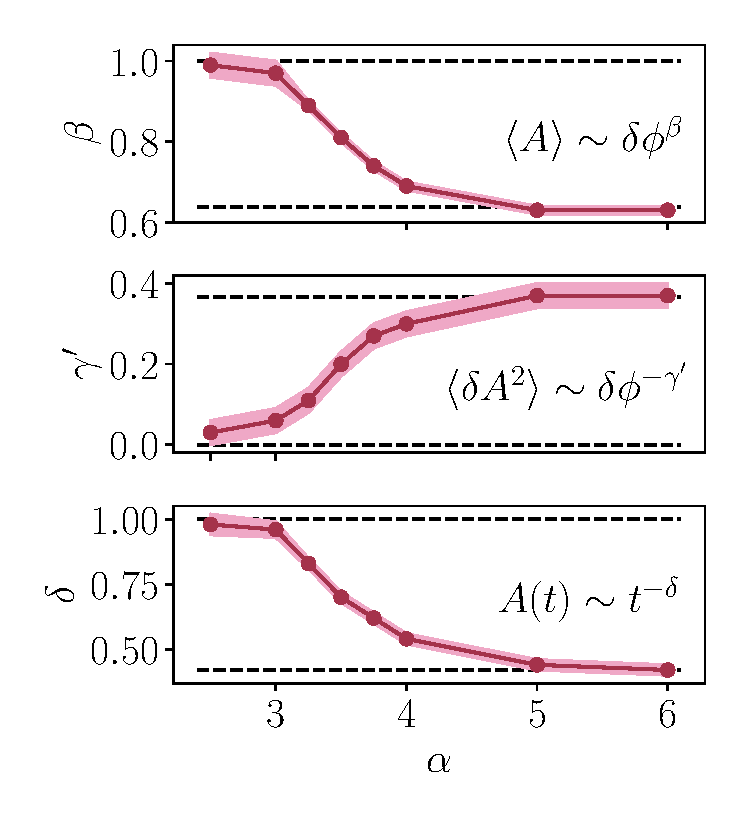
\includegraphics[width=0.6\textwidth]{Chapitre2/Figures/Exposants/exp_suspensions_jumps.pdf}
	\caption{Évolution des exposants critiques $\beta$, $\gamma^\prime$ et $\delta$  avec la portée dans les modèles LR-ROM. Les zones colorées en rose représentent les incertitudes de détermination.}
	\label{fig:EvolExpJumps}
\end{figure}

\subparagraph{}Finalement, l'estimation des exposants critiques dans le modèle LR-ROM confirme l'inscription des interactions de transport à longue portée dans le cadre théorique LR-CDP présenté à la \autoref{sec:LRCanonique}. En augmentant la portée du transport de matière dans le système, la criticalité passe continûment de son équivalent de courte portée à son équivalent de champ moyen, gardant une évolution concave du paramètre d'ordre ($\beta < 1$) et une divergence des fluctuations à l'approche du point critique ($\gamma^\prime>0$). Au premier ordre, cette évolution prend effectivement place dans la zone $3D/2 < \alpha < D+2$ soit $3<\alpha<4$ dans le cas bidimensionnel.

\begin{table}[h]
\centering
\begin{tabular}{cccccc}
\hline \hline $\alpha$ & $\beta$ & $\gamma^\prime$ & $\delta$ & $\nu_\perp^*$ & $\nu_\perp^\text{CM}$\\
\hline \text{CDP} \cite{lubeck_universal_2004} & 0.64 & 0.37 & 0.42 & 0.80 & 0.50\\
6 & 0.63 & 0.37 & 0.42 & 0.82 & 0.50\\
5 & 0.63 & 0.37 & 0.44 & 0.82 & 0.50\\
4 & 0.69 & 0.30 & 0.54 & 0.84 & 0.50\\
3.75 & 0.74 & 0.27 & 0.62 & 0.88 & 0.57\\
3.5 & 0.81 & 0.20 & 0.70 & 0.91 & 0.67\\
3.25 & 0.89 & 0.11 & 0.83 & 0.95 & 0.80\\
3 & 0.98 & 0.06 & 0.96 & 1.01 & 1.00\\
2.5 & 0.99 & 0.03 & 0.98 & - & 2.00\\
\hline \hline
\end{tabular}
\caption{Exposants critiques $\beta$, $\gamma^\prime$ et $\delta$ déterminés dans les modèles LR-ROM en 2D. La troisième colonne représente l'exposant $\nu_\perp$ dérivé par la relation d'échelle (\autoref{eq:HyperScaling}) et la quatrième l'exposant champ moyen associé à chaque portée $\alpha$.}
\label{tab:expocrit_LRROM}
\end{table}

\section{Hyperuniformité}

\subparagraph{}Dans cette dernière section, nous proposons de conclure la caractérisation quantitative du cadre théorique LR-CDP en 2D en nous intéressant à l'évolution de l'hyperuniformité. Dans la \autoref{sec:LRCanonique}, nous avons vu que dans ce cadre nous attendions une évolution continue de l'exposant d'hyperuniformité $\sigma$ entre $\alpha = 4$ et $\alpha=3$. Dans la limite de courte portée $\alpha \geq 4$, la théorie développée par mapping avec la transition de dépiégeage \cite{wiese_hyperuniformity_2024} prédit $\sigma = 0.75$ tandis qu'elle prédit $\sigma = 1$ pour $\alpha < 3$. Entre ces deux limites, des calculs issus du groupe de renormalisation fonctionnel permettent de prédire l'évolution de l'exposant $\sigma$ avec $\alpha$. Dans la suite de cette étude, nous proposons de confronter ces calculs théoriques via la caractérisation des propriétés hyperuniformes des modèles LR-ROM et LR-Manna pour différentes portées de transport $\alpha$. Ce travail, mené en collaboration étroite avec K. Wiese, est encore au stade préliminaire mais les premiers résultats associés soulèvent des points intéressants qu'il semble judicieux de faire figurer dans cette thèse, bien qu'ils n'en constituent pas l'objet principal. Notamment, nous montrons que les mesures d'hyperuniformité dans ces modèles se révèlent particulièrement exigeantes.

\label{sec:HUjumps}

\subsection{Hyperuniformité dans le LR-ROM}

\subparagraph{}En utilisant la méthode de box-counting présentée à la \autoref{sec:MethodHU}, nous commençons par caractériser les propriétés hyperuniformes des transitions du LR-ROM pour $\alpha\in\{ 5, 4, 3.75, 3.5, 3.25, 3 \}$. Afin d'opérer une comparaison juste entre toutes ces portées, nous étudions chacune d'elle pour une distance similaire au point critique $\delta\phi \approx 1\times 10^{-3}$ et une taille de système $L=4096$.

\begin{figure}[h]
	\centering	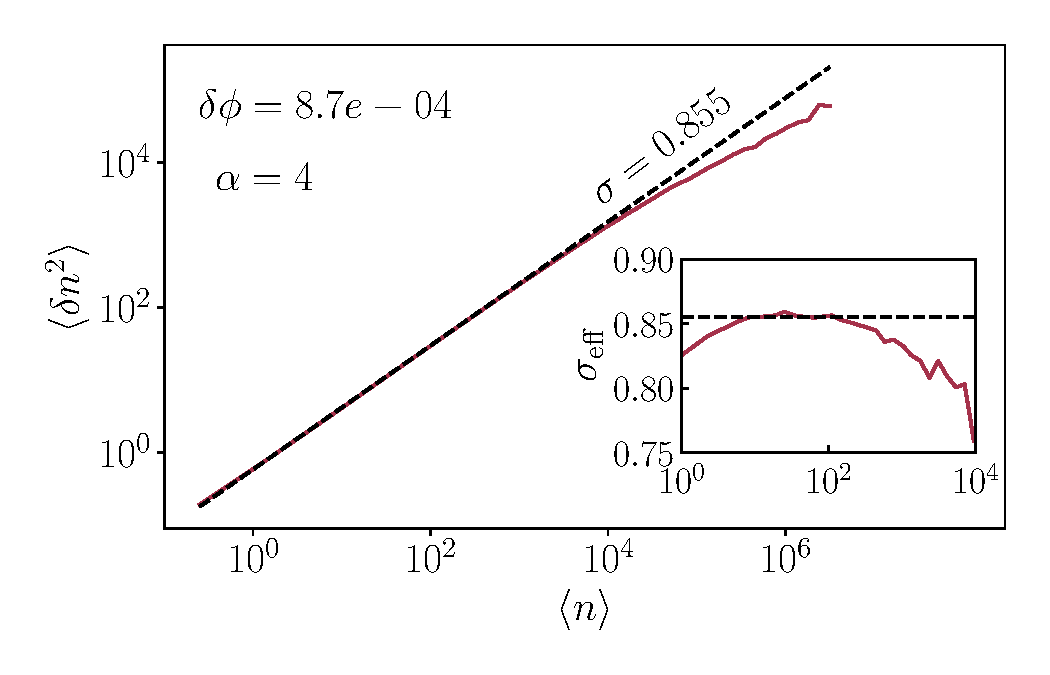
\includegraphics[width=0.65\textwidth]{Chapitre2/Figures/Hyperuniformity/FigHULRROM.pdf}
	\caption{Estimation de l'exposant d'hyperuniformité $\sigma$ dans le LR-ROM pour $\alpha=4$. En encart, l'exposant effectif local, déterminé comme la dérivée logarithmique de la courbe représentée en figure principale.}
	\label{fig:ExHUJumps}
\end{figure}

\subparagraph{}Nous présentons un exemple de mesure obtenue pour $\alpha=4$ à la \autoref{fig:ExHUJumps}. Une manière plus fine d'analyser ces résultats est de calculer la dérivée logarithmique de la courbe $\langle \delta n^2 \rangle = f(\langle n \rangle)$, afin d'obtenir une mesure de l'exposant effectif $\sigma_\text{eff}$ dépendante de l'échelle de longueur considérée. Celle-ci est représentée dans l'encart de la même figure. Comme nous l'avons mentionné précédemment, les propriétés universelles d'hyperuniformité sont valables entre deux crossovers : un de petite échelle (détails microscopiques non-universels) et un de grande échelle\footnote{En théorie il existe une troisième limite à ces mesures, provenant de la taille finie du système. En fait pour une taille de sous-compartiment proche de la taille du système, même pour un système hyperuniforme à toutes les échelles de longueur, l'évolution  $\langle \delta n^2 \rangle = f(\langle n \rangle)$ opère une décroissance. Cela se reflète dans le fait que pour $\langle n \rangle = N$ on a $\langle \delta n^2 \rangle =0$. Dans le cas d'une distribution poissonienne des positions cette décroissance est représentée par :

\begin{equation}
	 \langle \delta n^2 \rangle  = \langle n \rangle \left( 1-\frac{\langle n \rangle}{N} \right).
\end{equation}

\noindent Si cette limite de grande échelle se retrouve bien dans nos données, celle-ci se situe toujours à des échelles bien plus grandes que celle définie par la distance finie au point critique. Ainsi, nous n'avons pas besoin de nous préoccuper de cet effet en pratique.} (distance finie du point critique). Afin de déterminer $\sigma$, nous devons donc nous situer entre ces deux limites. Le choix que nous faisons pour l'estimation de $\sigma$ est alors de retenir la valeur de l'exposant effectif dans la zone sur laquelle il varie très peu, i.e. entre la croissance à petite échelle et la décroissance à grande échelle. Dans l'exemple de la \autoref{fig:ExHUJumps}, celle-ci se situe entre $\langle n \rangle \approx 10$ et $\langle n \rangle \approx 1000$ et donne $\sigma\approx 0.855$.

\subparagraph{}En appliquant la même procédure pour les différentes portées $\alpha$, nous obtenons l'évolution des exposants d'hyperuniformité présentée à la \autoref{fig:ExpTBLRJHU}, mise en comparaison avec les résultats théoriques \cite{wiese_longrange}. Nous remarquons alors que pour $3.25 < \alpha < 3.75$ les mesures sont très proches de l'attendu théorique. Toutefois, il existe un fort désaccord entre théorie et simulations pour les plus courtes portées $\alpha \geq 4$. En effet, nous attendons dans cette zone un plateau à $\sigma = 0.75$. Or ici, pour $\alpha \geq 4$, $\sigma$ semble encore diminuer légèrement avec $\alpha$ et prend des valeurs significativement plus grandes que $\sigma = 0.75$. D'autre part, la valeur $\sigma \approx 0.96$ pour $\gamma = 3$ est aussi légèrement différente de l'attendu champ moyen $\sigma = 1$. Malgré cela, nous retrouvons bien la tendance générale d'une hyperuniformité progressivement perdue avec l'augmentation de la portée du transport. Dans la suite de cette section, nous proposons des explications aux désaccords entre les résultats préliminaires obtenus dans le cadre de la caractérisation du LR-ROM et la théorie issue des calculs du groupe de renormalisation fonctionnel.

\begin{figure}[h]
	\centering	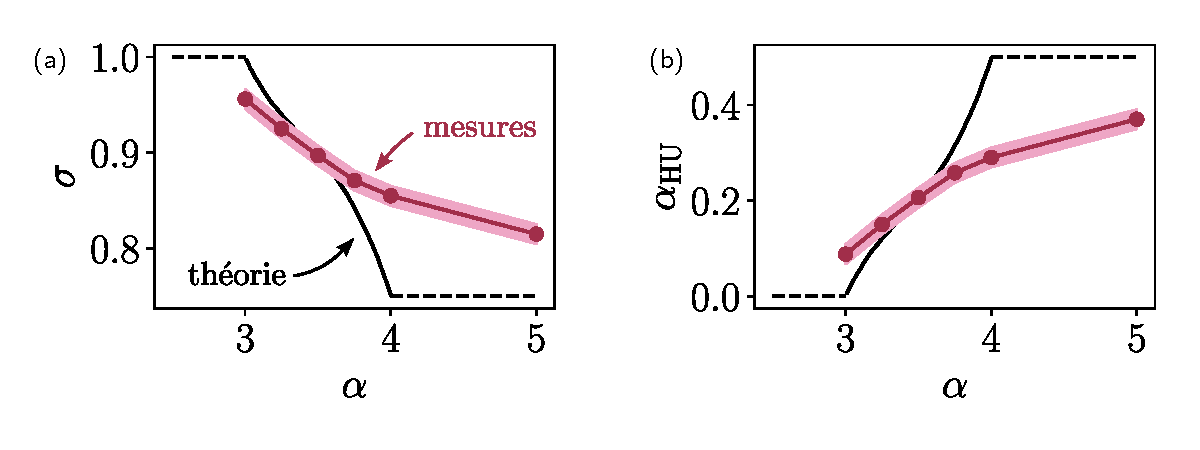
\includegraphics[width=0.9\textwidth]{Chapitre2/Figures/Hyperuniformity/eta_alpha_jumps.pdf}
	\caption{(a) Évolution de l'exposant d'hyperuniformité $\sigma$ avec la portée dans les modèles LR-ROM. La courbe noire représente les prédictions théoriques \cite{wiese_hyperuniformity_2024, wiese_theory_2022, wiese_longrange}. Les zones colorées rose représentent les incertitudes de détermination. (b) Déduction de l'évolution de l'exposant $\alpha_\text{HU}$ se basant sur l'\autoref{eq:eqsigmaalphahu}.}
	\label{fig:ExpTBLRJHU}
\end{figure}

\subsection{Difficultés dans les mesures d'hyperuniformité}

\subsubsection{Importance de la conservation du centre de masse}

\subparagraph{}Une première explication à ces différences vient du mouvement du centre de masse du système. En effet, dans la théorie de champ associée à CDP permettant d'effectuer les prédictions pour $\sigma$ présentées précédemment, le centre de masse du système est une quantité conservée \cite{wiese_blabla}. Or dans le LR-ROM, les sauts aléatoires des particules actives ne conservent ce centre de masse qu'en moyenne, leur direction étant complètement aléatoire. La rupture de cette symétrie fondamentale, directement reliée à la répartition des particules dans le système, pourrait donc affecter nos mesures de l'hyperuniformité et expliquer un désaccord avec les prédictions du cadre LR-CDP.

\subparagraph{}La façon la plus simple de le remarquer est de se placer dans le cas de la courte portée. Prenons le modèle Manna, appartenant à la classe CDP, et considérons deux de ses représentations. Dans la première représentation du modèle, l'implémentation est faite de la manière décrite à la \autoref{sec:ImplementationManna}, i.e. avec une redistribution aléatoire des particules sur les sites voisins. Celle-ci ne conserve donc pas le centre de masse du système. Dans la seconde représentation, lorsqu'un site est actif, il redistribue aléatoirement (i.e. dans une des deux directions principales du plan) une paire de particules sur deux sites voisins opposés, de manière à conserver le centre de masse du système à chaque instant. En effectuant alors des mesures sur ces deux représentations dans des configurations équivalentes avec $L=4096$ et $\langle A \rangle \approx 2\times 10^{-3}$, nous obtenons les résultats présentés à la \autoref{fig:HUCM}-(a)-(b).

\begin{figure}[h]
	\centering
	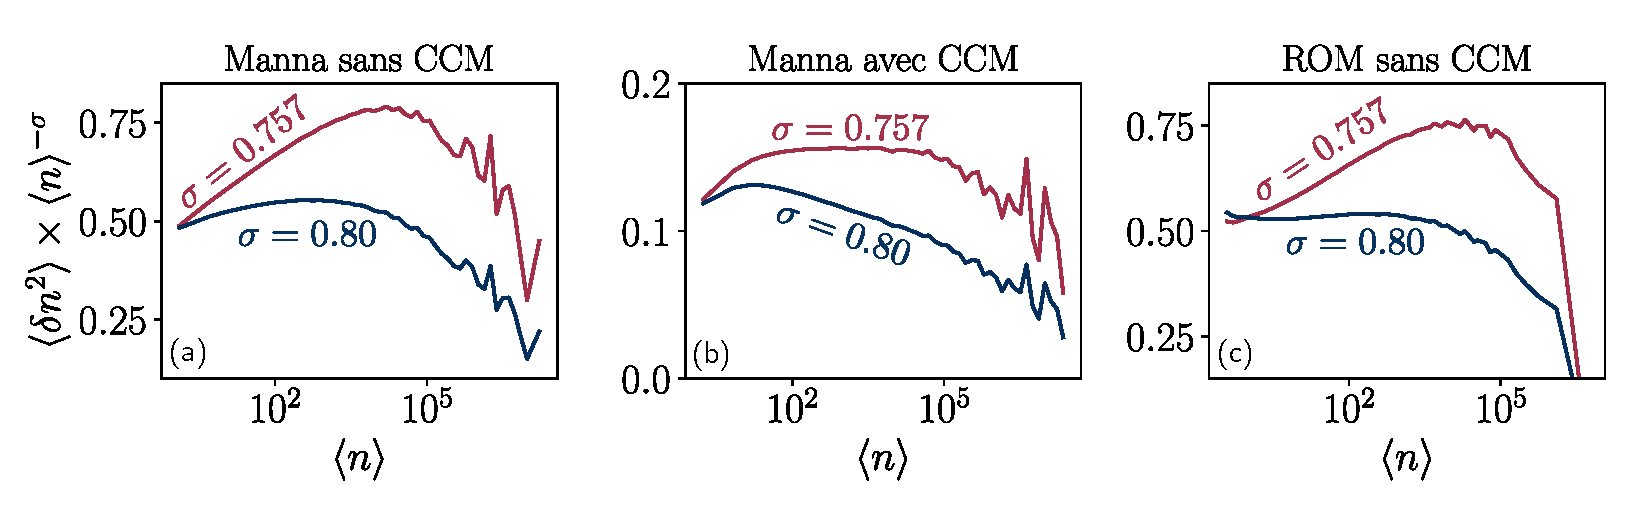
\includegraphics[width=\textwidth]{Chapitre2/Figures/Hyperuniformity/ImportanceCMHU.pdf}
	\caption{Représentation compensée de l'évolution de $\langle \delta n^2 \rangle$ avec $\langle n \rangle$ par une loi de puissance test dans (a) le modèle Manna 2D sans conservation de la position du centre de masse ($\phi = 1.30628$), (b) le modèle Manna 2D avec conservation de la position du centre de masse ($\phi = 1.75895$) et (c) le ROM 2D ($\phi = 0.235248$). Les courbes rouges représentent la compensation par l'exposant test $\sigma = 0.757$, adéquate pour le modèle conservant la position du centre de masse, et les courbes bleues représentent la compensation par l'exposant test $\sigma = 0.80$, adéquat pour les modèles ne conservant pas la position du centre de masse.}
	\label{fig:HUCM}
\end{figure}

\subparagraph{}En représentant l'évolution $\langle \delta n^2 \rangle = f(\langle n \rangle)$ compensée par une loi test\footnote{Cette méthode de mesure est similaire à celle de la dérivée logarithmique mais permet de travailler avec des signaux plus bruités.} $\langle n \rangle^\sigma$, ces mesures nous permettent d'estimer deux exposants distincts pour chacune des représentations : $\sigma \approx 0.76$ dans le cas où le centre de masse est conservé et $\sigma\approx 0.80$ dans le cas où il ne l'est pas. Dans le cas du ROM (donc avec des sauts courts) sans conservation du centre de masse, nous mesurons aussi dans ces mêmes conditions $\sigma\approx 0.80$, comme présenté à la \autoref{fig:HUCM}-(c).

\subparagraph{}Ces résultats suggèrent donc que la conservation du centre de masse joue un rôle essentiel dans les propriétés hyperuniformes du système. Notamment lorsque celle-ci est bafouée, il semble que cela revient à surestimer l'exposant $\sigma$ et donc diminuer l'hyperuniformité dans le système. Cela explique en partie pourquoi, dans le cas du LR-ROM, nous obtenons à $\alpha = 4$ une mesure de $\sigma\approx 0.86$ significativement plus grande que la valeur attendue $\sigma= 0.75$. Toutefois, cette valeur reste encore relativement éloignée de la valeur $\sigma\approx 0.80$ obtenue ici dans la limite de courte portée. Une explication à cette différence subsistante pourrait venir de la taille finie des systèmes étudiés.

\subsubsection{Effet de taille finie}

\subparagraph{}Si la loi de distribution des sauts des particules actives est une loi de puissance parfaite grâce à notre méthode de génération, en pratique elle se retrouve modifiée par sa mise en place dans un système de taille finie. En effet, par application des conditions aux limites périodiques, tous les sauts de taille $\Delta \gtrsim L$ se voient "repliés" dans l'espace périodique, changeant ainsi la distribution effective des sauts des particules actives. De plus, cette loi algébrique n'est définie que pour $\Delta>1$, du fait de l'introduction d'une distance de saut minimale lors de l'implémentation numérique.

\subparagraph{}Dans les approches théoriques permettant la prédiction de l'exposant $\sigma$, l'interaction à longue portée est considérée dans l'espace réciproque \cite{wiese_longrange}. Dans l'hypothétique système parfait et infini sur lequel se basent ces prédictions, la transformée de Fourier de la distribution de taille des sauts est définie par :

\begin{equation}
	\hat{P}_\Delta(q) \sim 1-|q|^{\alpha-D},
\end{equation}

\noindent soit correspondant à la fonction caractéristique d'une loi stable $S_{\alpha-D}$ dans la limite de petit $q$\footnote{Dans le cas d'une loi stable $S_{\alpha-D}$ on a en effet $\hat{P}_\Delta(q) \sim \text{exp}\left( -|q|^{\alpha-D} \right)$.}. Une hypothèse est alors que dans nos simulations, dû à la taille finie du système et à l'introduction d'un cut-off, les distributions s'éloignent de cet attendu par l'addition de termes réguliers dans le développement de la fonction caractéristique :

\begin{equation}
	\hat{P}_\Delta(q) \sim 1-|q|^{\alpha-D} + q^2 + ...
	\label{eq:DevStable}
\end{equation}

\noindent Le premier terme régulier en $\sim q^2$ est sous-dominant pour $\alpha < D+2$. Cependant à mesure que $\alpha \rightarrow D+2$, soit $\alpha\rightarrow 4$ dans notre cas, cette sous-dominance n'est effective que dans un domaine de $q$ de plus en plus petits et donc des systèmes de tailles de plus en plus grandes. Ainsi, proche de $\alpha = 4$, on pourrait s'attendre à ce que la distribution de sauts effective s'écarte significativement la distribution utilisée dans la théorie.

\begin{figure}[h]
	\centering
	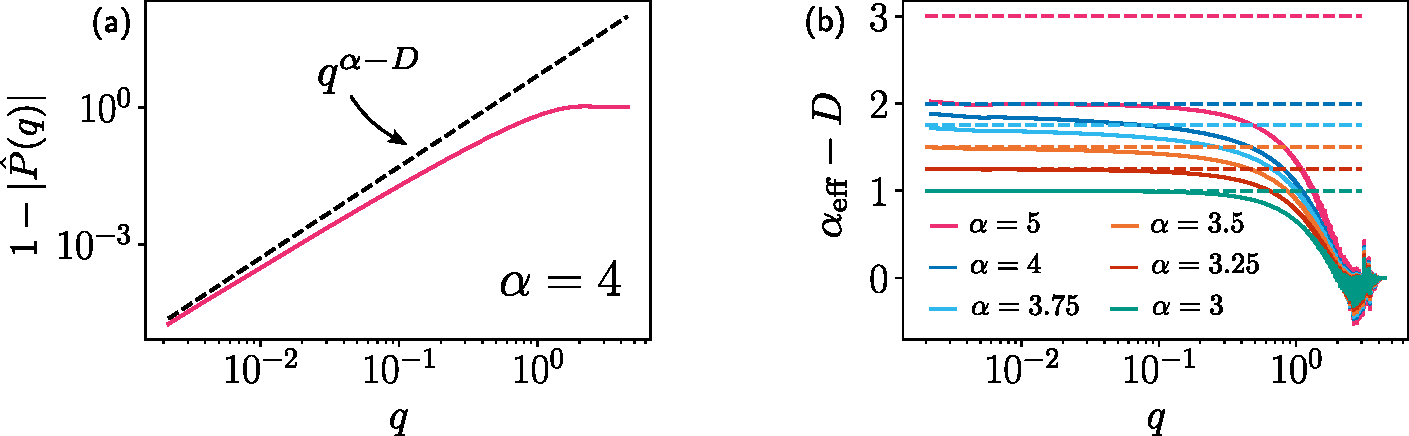
\includegraphics[width=\textwidth]{Chapitre2/Figures/Hyperuniformity/GammaEff_ROM.pdf}
	\caption{(a) Évolution de la quantité $1-|\hat{P}_\Delta (q)|$ avec $q$ pour le LR-ROM avec $\alpha=4$. En pointillé noir, le cas idéal sur lequel se basent les prédictions théoriques. (b) Exposant effectif obtenu par dérivée logarithmique de la courbe représentée en (a) pour toutes les portées $\alpha$. En pointillés de même couleur, la valeur $\alpha-D$ associée.}
	\label{fig:GammaEffROM}
\end{figure}

\subparagraph{}Pour le vérifier, nous considérons le cas du LR-ROM pour $L=4096$, dans lequel nous mesurons la distribution de probabilité $P(\mathbf{r})$ d'effectuer un déplacement $\mathbf{r}$ dans le système suite à un saut actif. En pratique nous en réalisons l'histogramme sur la grille introduite précédemment dans le cadre de la méthode cell-list. En prenant la transformée de Fourier discrète bidimensionnelle de cette distribution nous obtenons par une moyenne isotrope un équivalent de la distribution recherchée $\hat{P}_\Delta (q)$. Sur la \autoref{fig:GammaEffROM}, nous représentons $1-|\hat{P}_\Delta (q)|$ en fonction de $q$ pour $\alpha=4$ et la dérivée logarithmique obtenue de ces courbes pour chaque $\alpha$, définissant alors un exposant effectif local $\alpha_\text{eff}$. Pour chacune de ces portées, nous représentons en pointillés l'hypothèse théorique d'un exposant $\alpha-D$.

\subparagraph{}Nous observons alors effectivement une déviation de l'idéal théorique, d'autant plus que $\alpha$ se rapproche de $\alpha = 4$. De plus, pour $\alpha=5$, nous obtenons un exposant effectif $\alpha_\text{eff}\approx2$, signe de la prédominance du terme en $q^2$ dans l'\autoref{eq:DevStable} proposée précédemment, justifiant de ce fait notre raisonnement.
\`A la vue de ces observations, il est donc possible que les propriétés d'hyperuniformité du système soient effectivement affectées par les détails de l'implémentation des sauts à longue portée, et ce d'autant plus que $\alpha$ est proche de $\alpha=4$. Ceci, conjointement à la propriété de non-conservation de la position du centre de masse, pourrait expliquer le désaccord avec la théorie des résultats préliminaires obtenus dans le cas du LR-ROM.

%Afin de corriger cette dépendance, nous proposons une méthode de détermination d'un exposant de portée effectif $\alpha_\text{eff}$ équivalent à celui d'un système de taille infinie pour chaque portée $\alpha$. Cette méthode est bien sûr critiquable mais représente l'avancée actuelle de notre réflexion. Pour déterminer l'exposant effectif, nous opérons une moyenne logarithmique en fonction de $q$ de la dérivée logarithmique de $\hat{P}_\Delta(q)$ sur la zone $q<q_c$. Cette approche est motivée par la philosophie de calcul du groupe de renormalisation fonctionnel, dans laquelle chaque échelle de $q$ compte de manière équivalente. Le cut-off $q_c$ est alors choisi pour ignorer les effets de la dynamique microscopique du système. Pour ces mesures, nous faisons le choix arbitraire $q_c=xx$.
%
%\subparagraph{}Par cette méthode, il est possible d'associer à chaque portée $\alpha$ un exposant effectif $\alpha_\text{eff}$ permettant de resituer les résultats précédents. La courbe bleue sur la \textbf{Fig XX} montre alors les modifications apportées. Globalement, cette analyse permet de rationaliser en partie les écarts observés à courte portée, les associant à des exposants effectifs plus faibles. Toutefois, dans le cas du LR-ROM, la non conservation du centre de masse reste un élément de désaccord. Afin de conclure cette étude, nous proposons de poursuivre notre étude sur un modèle conservant la position de celui-ci.

\subsection{Hyperuniformité dans le modèle LR-Manna}

\subsubsection{Résultats préliminaires}

\subparagraph{}Pour aller un peu plus loin, nous proposons d'étudier l'hyperuniformité dans les modèles de transport à longue portée au plus proche possible des conditions d'applications des prédictions théoriques afin de les confronter directement. Pour ce faire, nous considérons le modèle LR-Manna dans sa version qui inclue la conservation de la position du centre de masse. Ce choix n'est pas anodin. Ce modèle étant plus simple que le LR-ROM, il est plus aisé dans ce cas de considérer des tailles de systèmes plus grandes, et ainsi se rapprocher de la limite théorique de système infini. Nous appliquons alors la méthode de box-counting sur des systèmes allant jusqu'à des tailles $L=16384$ et des distances au point critique allant jusqu'à $\delta\phi \approx 5\times 10^{-5}$ pour chaque portée $\alpha\in\{ 4, 3.75, 3.5, 3.25, 3 \}$. La \autoref{fig:MannaCMHU_gamma4} présente les résultats obtenus pour $\alpha = 4$ pour toutes les densités considérées.

\begin{figure}[h]
	\centering
	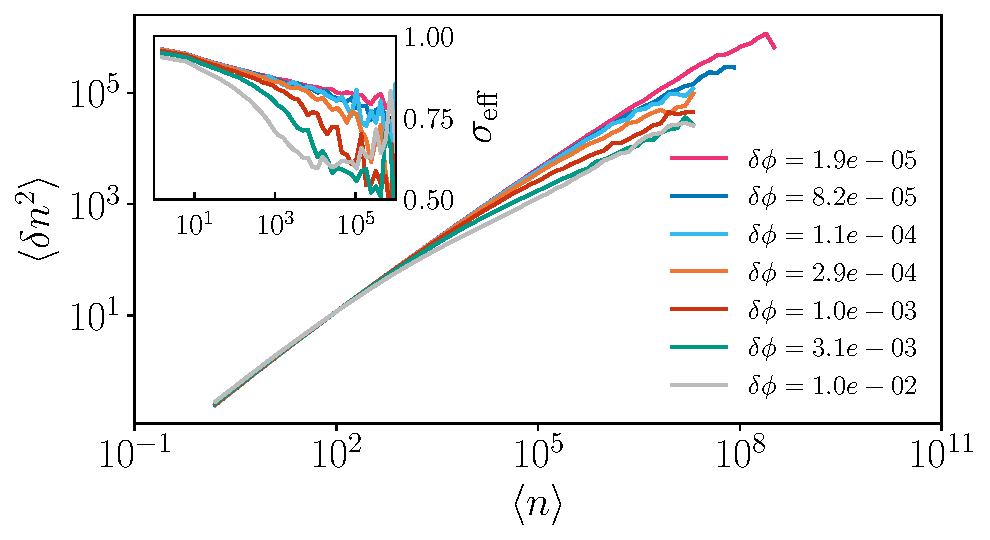
\includegraphics[width=0.9\textwidth]{Chapitre2/Figures/Hyperuniformity/MannaCM_gamma4_results.pdf}
	\caption{Évolution de $\langle \delta n^2 \rangle$ avec $\langle n \rangle$ dans le cas du modèle LR-Manna avec conservation de la position du centre de masse pour $\alpha=4$ à différentes distances $\delta\phi$ du point critique. En encart, l'évolution de l'exposant effectif mesuré par dérivation logarithmique des courbes en figure principale.}
	\label{fig:MannaCMHU_gamma4}
\end{figure}

\subparagraph{}Dans l'encart de cette figure, nous représentons l'exposant effectif local $\sigma_\text{eff}$ obtenu par dérivation logarithmique des courbes en figure principale. De manière assez surprenante, celui-ci semble évoluer de manière significative avec l'échelle de longueur considérée. Plus précisément, cette dépendance avec $\langle n \rangle$ semble être presque logarithmique, voire une loi de puissance de très faible exposant, jusqu'à un cut-off dépendant de la distance au point critique $\delta\phi$. Plus le système est proche du point critique, plus cette décroissance s'étend sur une large gamme d'échelles de longueurs. Pour la distance la plus proche du point critique étudiée $\delta\phi\approx 2\times 10^{-5}$, il semblerait que cette évolution commence tout juste à arriver à saturation à grande échelle (léger début d'inflexion de la courbe) avant l'apparition du cut-off, suggérant le début d'une convergence vers la valeur asymptotique $\sigma$ de la limite thermodynamique de grande échelle.

\subparagraph{}Cette analyse des données préliminaires ne permet donc pas la mesure d'un exposant unique dans la limite de grande échelle et suggère qu'une meilleure approche du point critique est nécessaire pour cela. Les modèles Manna et ROM étant dans la même classe d'universalité, nous pouvons considérer qu'il en est en fait de même pour les données présentées à la \autoref{fig:ExpTBLRJHU}. Ceci expliquerait une partie du désaccord avec la prédiction théorique, notamment le fait que pour $\alpha=4$, nos mesures ne convergent pas vers celles obtenues à courte portée.

\subparagraph{}Dans le cadre du modèle LR-Manna, en prenant l'exemple de la portée $\alpha=4$ et en considérant qu'à taille de système infinie nous attendons $\sigma=0.75$, l'analyse de ces données suggère que le régime algébrique est atteint, pour un système infini, pour $\langle n \rangle^* \gg 2\times 10^7$ soit $l^* \gg 4\times 10^3$. Afin de le mesurer directement, il faudrait donc parvenir à sonder un état pour lequel la longueur de corrélation $\xi$ associée est telle que $\xi\gg l^*$. Or, avec les ressources actuellement à notre disposition, nous pouvons difficilement envisager des tailles de systèmes $L>16384$ et donc atteindre une telle longueur de corrélation sans tomber dans un état absorbant. 

\subparagraph{}Dans le cas des plus grandes portées $\alpha<4$, l'analyse est parfois un peu moins défavorable (essentiellement pour le cas $\alpha = 3$) mais conserve les mêmes conclusions. Dans la suite, en nous basant sur ces observations préliminaires, nous proposons une piste permettant une estimation de l'exposant d'hyperuniformité $\sigma$ de la limite thermodynamique à chaque portée, ou à défaut une borne supérieure raisonnable de son encadrement.

\subsubsection{Perspectives}

\subparagraph{}Comme nous l'avons présenté précédemment, une manière de mesurer efficacement l'hyperuniformité dans un système est de procéder à une méthode de redimensionnement par la distance au point critique. En suivant \cite{hexner_hyperuniformity_2015}, nous redimensionnons donc la dimension de la boîte de comptage $l$ par $\delta\phi^{-\nu_\perp^*}$, $\nu_\perp^*$ étant l'exposant de corrélation spatiale dérivé précédemment de la relation d'hyperscaling. Cela revient alors à redimensionner $\langle n \rangle_l$ par $\delta\phi^{-D \nu_\perp^*} = \delta\phi^{-2\beta-\gamma^\prime}$. Parallèlement, nous redimensionnons $\langle \delta n^2 \rangle$ par $\delta\phi^a$ avec $a$ un exposant test afin d'espérer une superposition des courbes sur une courbe maîtresse. Ce faisant, il n'est en pratique pas aisé de déterminer un critère de bonne superposition puisque cette dernière n'est possible que localement. Pour s'en apercevoir, un exemple de redimensionnement pour $\alpha=4$ est donné sur la \autoref{fig:MannaCMHU_rescale_gamma4}-(a), dans lequel nous avons essayé de superposer la région à grand $\langle n \rangle$. Une méthode de cette nature ne semble donc pas pouvoir nous informer davantage.

\subparagraph{}Toutefois, si nous opérons la même procédure sur l'exposant effectif (i.e. la dérivée logarithmique de ces courbes), il est possible de superposer toutes ses évolutions sur une courbe maîtresse. Un exemple est donné dans le cas $\alpha=4$ sur la \autoref{fig:MannaCMHU_rescale_gamma4}-(b) et le cas des autres portées est relégué dans l'\annexeref{sec:mesures_HU_Manna}. De cette façon, il est possible d'en déduire précisément l'évolution algébrique de $\sigma_\text{eff}$ avec $\langle n \rangle$. Par ailleurs, nous remarquons que pour les distances $\delta\phi$ les plus petites, les courbes semblent s'éloigner légèrement, en moyenne, de cette superposition\footnote{Cette observation reste discutable du fait du bruit présent sur ces données préliminaires.}. Cet écart correspondrait alors au début de saturation vers l'exposant asymptotique déjà suggéré par les données brutes. En d'autres termes, il semblerait que l'exposant effectif suive une évolution du type :

\begin{equation}
	\sigma_\text{eff}  = \left( \sigma + \langle n \rangle^{-x} \right)g\left( \frac {\langle n \rangle }{\langle n \rangle_c} \right), \quad \langle n \rangle_c \sim \delta\phi^{-D\nu_\perp},
	\label{eq:esposantHULoi}
\end{equation}

\noindent avec $g(y)$ constante pour $y \ll 1$ et à décroissance rapide pour $y>1$. En pratique nous mesurons un exposant $x < 0.02$, décroissant davantage avec l'augmentation de la portée de l'interaction et donc la diminution de $\alpha$. $\alpha=4$ constitue donc le cas de plus forte dépendance de $\sigma_\text{eff}$ avec $\langle n \rangle$ même si celle-ci reste très ténue. 

\begin{figure}[h]
	\centering
	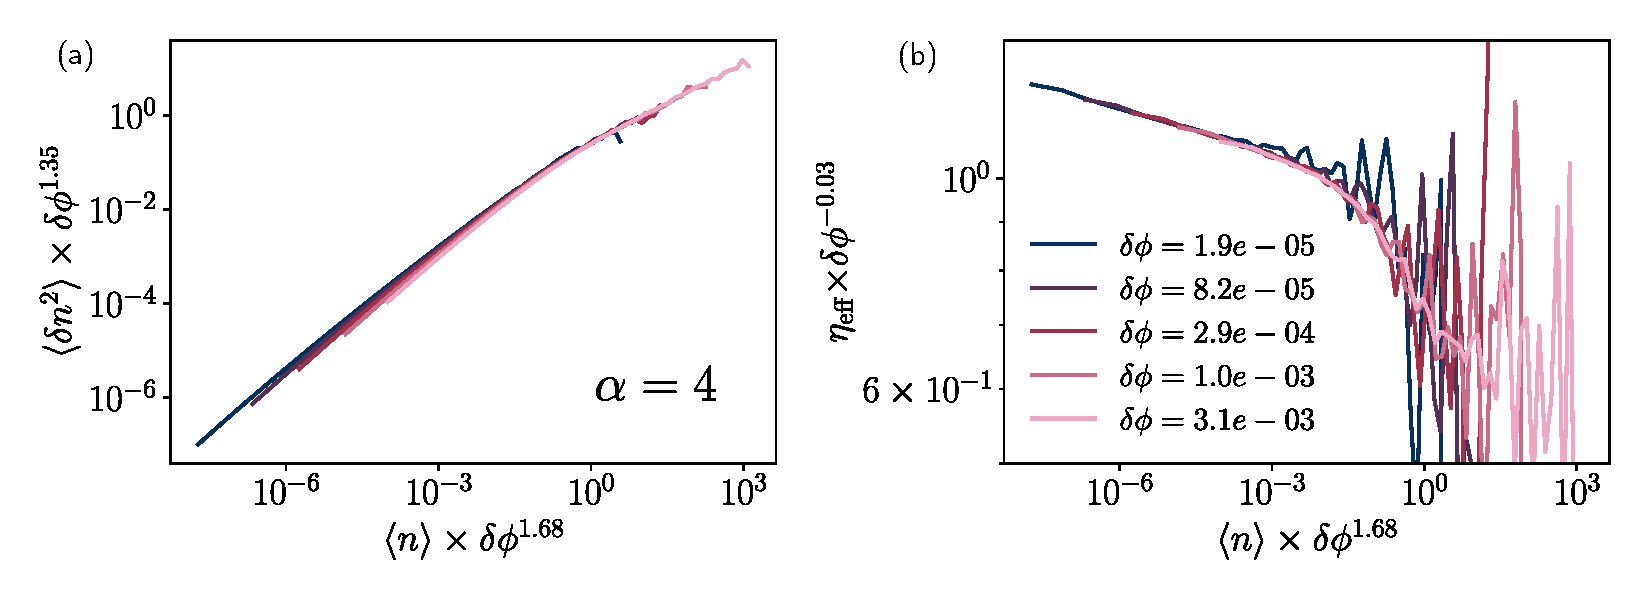
\includegraphics[width=\textwidth]{Chapitre2/Figures/Hyperuniformity/RescaleHU_MannaCM_Gamma4.pdf}
	\caption{Redimensionnement des mesures d'hyperuniformité dans le cas du modèle LR-Manna avec conservation de la position du centre de masse pour $\alpha=4$. Le redimensionnement par la distance au point critique $\delta\phi$ est appliqué sur (a) les données brutes et (b) l'exposant effectif obtenu par dérivée logarithmique.}
	\label{fig:MannaCMHU_rescale_gamma4}
\end{figure}

\subparagraph{}Cette méthode d'analyse, si elle ne nous permet pas de conclure sur la base de ces données préliminaires, présente un grand avantage : elle permet de déterminer sur une courbe $\langle  \delta n^2 \rangle  = f(\langle n \rangle )$ donnée la zone affectée par la distance finie au point critique considérée (i.e. l'influence du cut-off). Elle permet donc, si la forme donnée à l'\autoref{eq:esposantHULoi} est valide, de déterminer une borne supérieure sur l'encadrement de $\sigma$. En effet, dans ce cadre, tous les points sur la décroissance purement algébrique vérifient $\sigma_\text{eff}>\sigma$. Par ailleurs dans le cas le plus favorable $\alpha=3$ où la saturation vers l'exposant asymptotique semble être atteinte, nous pouvons estimer une valeur de $\sigma$, voire même une borne inférieure de l'encadrement. Ainsi, ces données préliminaires nous permettent de placer des indications de comparaison à la théorie sur la \autoref{eq:HUMannaShlag}. L'affinage nécessaire de ces estimations exige cependant un effort ultérieur.

\begin{figure}[h]
\centering
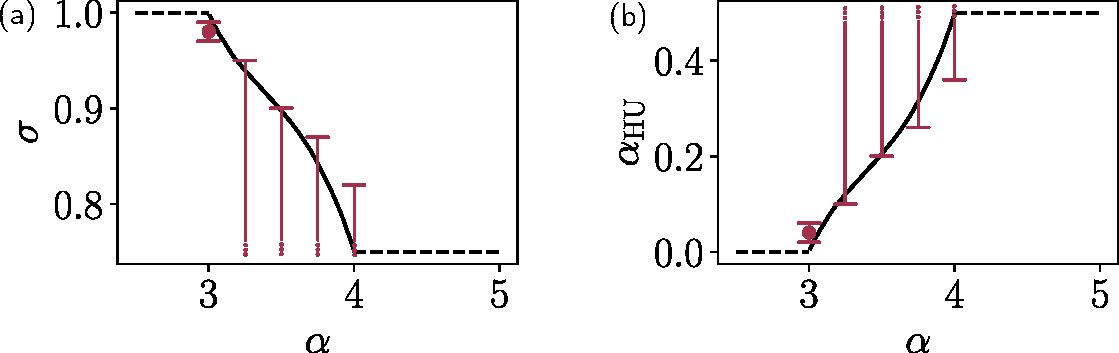
\includegraphics[width=0.8\textwidth]{Chapitre2/Figures/Hyperuniformity/eta_alpha_jumpsManna.pdf}
\caption{(a) Estimation de l'exposant d'hyperuniformité $\sigma$ dans le modèle LR-Manna avec conservation de la position du centre de masse pour les différentes portées $\alpha$. En pratique, il n'est possible d'encadrer et d'estimer la valeur de $\sigma$ que pour $\alpha=3$. Pour $\alpha>3$, nous proposons tout de même une borne supérieure de l'encadrement de cet exposant. En trait noir, les prédictions issues du mapping sur la transition de dépiégeage \cite{wiese_longrange}. (b) Déduction de l'évolution de l'exposant $\alpha_\text{HU}$ se basant sur l'\autoref{eq:eqsigmaalphahu}.}
\label{eq:HUMannaShlag}
\end{figure}

\subparagraph{}La détermination des propriétés hyperuniformes dans les modèles de sauts à longue portée exige donc de se placer à de très grandes échelles de longueur et donc des densités très proches du point critique. Il semble alors que c'est cette observation, plus que celle de la taille finie du système, ajoutée à celle concernant l'influence de la conservation du centre de masse, qui explique pourquoi nos mesures préliminaires dans le cadre du LR-ROM s'éloignent des prédictions théoriques. 

\subparagraph{}En conclusion, cette étude préliminaire révèle que les mesures de l'hyperuniformité dans ces modèles semblent relever d'une tâche très exigeante. La caractérisation quantitative des exposants $\sigma$ et leur évolution précise avec la portée $\alpha$ n'étant pas essentielles au reste de notre propos, nous nous limiterons à cette détermination au premier ordre. Celle-ci décrit alors, comme prédit par la théorie, une perte progressive de l'hyperuniformité dans le système avec l'augmentation de la portée de $\alpha=4$ à $\alpha=3$. La disparition de l'hyperuniformité pouvant être interprétée comme la disparition des corrélations spatiales de densité, cette observation est cohérent avec le fait que l'on rejoint un régime de champ moyen pour $\alpha <3$ dans le cadre LR-CDP. Ces éléments nous suffiront à contraster les évolutions observées en présence d'interactions médiées à longue portée dans les transitions de réversibilité et d'écoulement.

\subsubsection{Retour sur les exposants critiques}

\subparagraph{}La nécessité de s'approcher extrêmement près du point critique pour observer la criticalité de la limite thermodynamique pourrait aussi avoir un impact sur la détermination des exposants critiques présentée à la \autoref{sec:expcritjumps}. Cela pourrait expliquer pourquoi dans le cas identifié comme le plus défavorable $\alpha=4$, nous observons un écart à la limite de courte portée concernant les exposants $\beta$, $\gamma^\prime$ et $\delta$.

\subparagraph{}Toutefois, cette dépendance n'est pas évidente dans ces cas. En effet, sous un choix adéquat de densité critique $\phi_c$, les différentes lois de puissance déterminées sont bien plus convaincantes que celles obtenues par la méthode de box-counting dans le cadre de la mesure de l'hyperuniformité. Nous pouvons supposer par ailleurs que la conservation ou non de la position du centre de masse joue un rôle moins important dans le cas des exposants liés à l'activité dans le système ($\beta$, $\gamma^\prime$, $\delta$) plutôt qu'à la répartition de la masse ($\sigma$). Pour étudier ces hypothèses, il faudrait notamment sonder des états plus proches du point critique, requérant de fait une mobilisation de ressources numériques très importantes. Le but de ce travail étant essentiellement de caractériser une base de comparaison pour les études suivantes, nous nous limiterons aussi pour ces exposants à cette détermination de première ordre, tout de même relativement convaincante.

\section{Conclusion de chapitre}

\subparagraph{}Dans ce chapitre, nous avons défini le cadre théorique LR-CDP, représentant la présence d'un transport à longue portée induit localement par l'activité dans la classe CDP. Par une analyse d'échelle et des résultats pré-existants, nous avons prédit dans ce cadre l'évolution de la criticalité avec la portée des interactions $\alpha$. Notamment, en 2D, celle-ci prend place entre $\alpha=4$ et $\alpha=3$.


\subparagraph{}Pour préciser ce cadre, nous avons ensuite étudié des modèles emblématiques de la classe CDP auxquels nous avons ajouté un mécanisme de transport à longue portée. En caractérisant les transitions de phase absorbantes associées à chaque portée de transport, nous avons montré que les exposants critiques évoluent continûment avec la portée du transport, allant de leur équivalent de courte portée à leur équivalent de champ moyen. Au premier ordre, cette évolution se fait dans la gamme de portées effectivement prédite par la théorie LR-CDP.

\subparagraph{}Dans une seconde partie, nous avons présenté une étude préliminaire des propriétés d'hyperuniformité de ces systèmes et leur évolution avec la portée du transport. La détermination des exposants critiques dans ce cadre s'est alors révélée bien plus compliquée, montrant un écart avec les prédictions théoriques dont nous avons proposé deux explications complémentaires. La première vient de la conservation de la position du centre de masse qui est essentielle à la correspondance aux prédictions théoriques. La seconde vient d'un comportement pré-asymptotique s'étendant sur de très grandes plages d'échelles de longueur, rendant difficile l'estimation du comportement dans la limite thermodynamique.

\subparagraph{}En conclusion, cette étude nous a permis de préciser la zone flottante d'évolution des exposants critiques située entre $\alpha=3$ et $\alpha = 4$ en deux dimensions. Grâce à cet ajout, nous disposons d'un cadre mieux défini pour décrire l'évolution de la criticalité des systèmes sous l'ajout d'un transport à longue portée induit localement par l'activité. Dans la suite de cette thèse, nous nous servirons de cette base de comparaison afin de montrer que les interactions à longue portée, lorsqu'elles correspondent à des interactions médiées par le milieu non-équivalentes à un transport induit localement par l'activité, font évoluer la criticalité des systèmes d'une manière tout à fait différente.
